\RequirePackage[l2tabu, orthodox]{nag}
\documentclass[a4paper,twoside,10pt,DIV=12]{scrreprt}
\usepackage[stretch=10]{microtype}
\usepackage[american]{babel}
\usepackage[utf8]{inputenc}
\usepackage{amsmath}
\usepackage{amsfonts}
\usepackage[sc]{mathpazo}
\usepackage{hyperref}
\usepackage{url}
\usepackage{xspace}
\usepackage{dsfont}
\usepackage{mathabx}  % vDash
\usepackage{wasysym}
\usepackage{stmaryrd}
%\usepackage{showlabels}
\usepackage{tabulary}
\usepackage[numbers]{natbib}
\usepackage{rotating}
\usepackage{booktabs}
\usepackage{tikz}
\usepackage{calc}
\usetikzlibrary{backgrounds}
\usetikzlibrary{shadows}
\usetikzlibrary{arrows}
\pgfdeclarelayer{background}
\pgfdeclarelayer{foreground}
\pgfsetlayers{background,main,foreground}

\addtokomafont{caption}{\small}
\setkomafont{captionlabel}{\sffamily\bfseries}

% TODO
\usepackage{todonotes}
\newcommand{\stodo}[2][]
    {\todo[caption={#2},#1]
    {\footnotesize #2}}
\newcommand{\spottodo}[2][]{\stodo[color=green!40,caption={#2},#1]{#2}}
\newcommand{\ltltodo}[2][]{\stodo[color=red!40,caption={#2},#1]{#2}}

\newcommand{\uni}[1]{\texttt{\small U+#1}}

% For tables.
\newcommand{\newfootnotemark}[1]{\addtocounter{footnote}{#1}\footnotemark[\value{footnote}]}
\newcommand{\newfootnotetext}[2]{\addtocounter{footnote}{#1}\footnotetext[\value{footnote}]{#2}}


%% ---------------------- %%
%% Mathematical symbols.  %%
%% ---------------------- %%
\newcommand{\Z}{\texorpdfstring{\ensuremath{\mathds{Z}}}{Z}}
\newcommand{\B}{\texorpdfstring{\ensuremath{\mathds{B}}}{B}}
\newcommand{\N}{\texorpdfstring{\ensuremath{\mathds{N}}}{N}}
\newcommand{\AP}{\ensuremath{\mathrm{AP}}}

\DeclareMathOperator{\F}{\texttt{F}}
\DeclareMathOperator{\FALT}{\texttt{<>}}
\newcommand{\FREP}[1]{\texttt{F[#1]}}
\DeclareMathOperator{\G}{\texttt{G}}
\DeclareMathOperator{\GALT}{\texttt{[]}}
\newcommand{\GREP}[1]{\texttt{G[#1]}}
\newcommand{\U}{\mathbin{\texttt{U}}}
\newcommand{\R}{\mathbin{\texttt{R}}}
\newcommand{\RALT}{\mathbin{\texttt{V}}}
\DeclareMathOperator{\X}{\texttt{X}}
\newcommand{\XREP}[1]{\texttt{X[#1]}}
\DeclareMathOperator{\XALT}{\texttt{()}}
\newcommand{\M}{\mathbin{\texttt{M}}}
\newcommand{\W}{\mathbin{\texttt{W}}}
\DeclareMathOperator{\NOT}{\texttt{!}}
\DeclareMathOperator{\NOTALT}{\texttt{\char`~}}
\newcommand{\XOR}{\mathbin{\texttt{xor}}}
\newcommand{\XORALT}{\mathbin{\texttt{\char`^}}}
\newcommand{\IMPLIES}{\mathbin{\texttt{->}}}
\newcommand{\IMPLIESALT}{\mathbin{\texttt{=>}}}
\newcommand{\IMPLIESALTT}{\mathbin{\texttt{-->}}}
\newcommand{\EQUIV}{\mathbin{\texttt{<->}}}
\newcommand{\EQUIVALT}{\mathbin{\texttt{<=>}}}
\newcommand{\EQUIVALTT}{\mathbin{\texttt{<-->}}}
\newcommand{\OR}{\mathbin{\texttt{|}}}
\newcommand{\ORALT}{\mathbin{\texttt{||}}}
\newcommand{\ORALTT}{\mathbin{\texttt{\char`\\/}}}
\newcommand{\ORALTTT}{\mathbin{\texttt{+}}}
\newcommand{\AND}{\mathbin{\texttt{\&}}}
\newcommand{\ANDALT}{\mathbin{\texttt{\&\&}}}
\newcommand{\ANDALTT}{\mathbin{\texttt{/\char`\\}}}
\newcommand{\FUSION}{\mathbin{\texttt{:}}}
\newcommand{\CONCAT}{\mathbin{\texttt{;}}}
\newcommand{\DELAY}[1]{\mathbin{\texttt{\#\##1}}}
\newcommand{\DELAYR}[1]{\mathbin{\texttt{\#\#[#1]}}}
\newcommand{\DELAYP}[1]{\mathbin{\texttt{\#\#[+]}}}
\newcommand{\DELAYS}[1]{\mathbin{\texttt{\#\#[*]}}}
\newcommand{\0}{\texttt{0}}
\newcommand{\1}{\texttt{1}}
\newcommand{\STAR}[1]{\texttt{[*#1]}}
\newcommand{\FSTAR}[1]{\texttt{[:*#1]}}
\newcommand{\STARALT}{\texttt{*}}
\newcommand{\STARBIN}{\mathbin{\texttt{*}}}
\newcommand{\EQUAL}[1]{\texttt{[=#1]}}
\newcommand{\GOTO}[1]{\texttt{[->#1]}}
\newcommand{\PLUS}{\texttt{[+]}}
\newcommand{\FPLUS}{\texttt{[:+]}}
\newcommand{\FIRSTMATCH}{\texttt{first\_match}}
\newcommand{\eword}{\texttt{[*0]}}

\newcommand{\Esuffix}{\texttt{<>->}}
\newcommand{\EsuffixMarked}{\texttt{<>+>}}
\newcommand{\Asuffix}{\texttt{[]->}}
\newcommand{\AsuffixALT}{\texttt{|->}}
\newcommand{\EsuffixEQ}{\texttt{<>=>}}
\newcommand{\AsuffixEQ}{\texttt{[]=>}}
\newcommand{\AsuffixALTEQ}{\texttt{|=>}}

\newcommand{\sere}[1]{\texttt{\{}#1\texttt{\}}}
\newcommand{\nsere}[1]{\texttt{!\{}#1\texttt{\}}}
\newcommand{\nsereMarked}[1]{\texttt{!+\{}#1\texttt{\}}}
\newcommand{\seren}[1]{\texttt{\{}#1\texttt{\}!}}

% rewriting rules that enlarge the formula
\newcommand{\equiV}{\stackrel{\star}{\equiv}}
% rewriting rules that favors event/univ
\newcommand{\equivEU}{\stackrel{\blacktriangleup}{\equiv}}
\newcommand{\equivNeu}{\stackrel{\smalltriangledown}{\equiv}}

% marked rewriting rules
\newcommand{\equivM}{\stackrel{\dag}{\equiv}}

\def\limplies{\rightarrow}
\def\simpe{\rightleftharpoons}
\def\simp{\rightrightharpoons}
\def\Simp{\stackrel{+}{\simp}}
\def\liff{\leftrightarrow}

\makeatletter
\newcommand{\Cxx}{%
  \valign{\vfil\hbox{##}\vfil\cr
    {C\kern-.1em}\cr
    $\hbox{\fontsize\sf@size\z@\textbf{+\kern-0.05em+}}$\cr}%
    \xspace
}
\makeatother

\def\clap#1{\hbox to 0pt{\hss#1\hss}}
\def\mathllap{\mathpalette\mathllapinternal}
\def\mathrlap{\mathpalette\mathrlapinternal}
\def\mathclap{\mathpalette\mathclapinternal}
\def\mathllapinternal#1#2{%
           \llap{$\mathsurround=0pt#1{#2}$}}
\def\mathrlapinternal#1#2{%
           \rlap{$\mathsurround=0pt#1{#2}$}}
\def\mathclapinternal#1#2{%
           \clap{$\mathsurround=0pt#1{#2}$}}

% The same argument is output and put in the index.
\usepackage{makeidx}
\makeindex
\newcommand{\Index}[1]{\index{#1}#1}

% Tikz
\tikzstyle{annote}=[overlay,thick,<-,red,>=stealth']


% Make sure we can compile this file even without use the version
% supplied by the Makefile.
\ifdefined\SpotVersion\else
 \def\SpotVersion{\textbf{UNKNOWN VERSION}}
\fi

%% ----------------------- %%
%% Texinfo like commands.  %%
%% ----------------------- %%

\newcommand\file[1]{`\texttt{#1}'}
\newcommand\command[1]{\texttt{#1}}
\newcommand\var[1]{{\ttfamily\itshape #1}}
\newcommand\mvar[1]{\ensuremath{\mathit{#1}}}
\newcommand\code[1]{\texttt{#1}}
\newcommand\samp[1]{`\texttt{#1}'}
\newcommand\tsamp[1]{\text{\texttt{#1}}}
\newcommand\msamp[1]{#1}


\def\manualtitle{Spot's Temporal Logic Formulas}

%% ---------- %%
%% Document.  %%
%% ---------- %%
\begin{document}

\vspace*{50pt}
\vskip4pt \hrule height 4pt width \hsize \vskip4pt
\begin{center}
  \huge \manualtitle
\end{center}
\vspace*{-1.5ex}
\vskip4pt \hrule height 4pt width \hsize \vskip4pt

\hfill Alexandre Duret-Lutz
\href{mailto:adl@lrde.epita.fr}{\nolinkurl{<adl@lrde.epita.fr>}}

\hfill compiled on \today, for Spot \SpotVersion

\vfill

\setcounter{tocdepth}{2}
\makeatletter
\@starttoc{toc}
\makeatother

\vfill

\chapter{Reasoning with Infinite Sequences}

\section{Finite and Infinite Sequences}

Let $\N=\{0,1,2,\ldots\}$ denote the set of natural numbers and
$\omega\not\in\N$ the first transfinite ordinal.  We extend the $<$
relation from $\N$ to $\N\cup\{\omega\}$ with $\forall n\in \N,\,
n<\omega$.  Similarly let us extend the addition and subtraction with
$\forall n\in\N,\,\omega+n = \omega-n = \omega+\omega = \omega$.

For any set $A$, and any number $n\in\N\cup\{\omega\}$, a
\textit{sequence} of length $n$ is a function $\sigma:
\{0,1,\ldots,n-1\}\to A$ that associates each index $i<n$ to an
element $\sigma(i)\in A$.  The sequence of length $0$ is a particular
sequence called the \textit{empty word} and denoted $\varepsilon$.  We
denote $A^n$ the set of all sequences of length $n$ on $A$ (in
particular $A^\omega$ is the set of infinite sequences on $A$), and
$A^\star=\bigcup_{n\in\N}A^n$ denotes the set of all finite sequences.
The length of any sequence $\sigma$ is noted $|\sigma|$, with
$|\sigma|\in\N\cup\{\omega\}$.

For any sequence $\sigma$, we denote $\sigma^{i..j}$ the finite
subsequence built using letters from $\sigma(i)$ to $\sigma(j)$.  If
$\sigma$ is infinite, we denote $\sigma^{i..}$ the suffix of $\sigma$
starting at letter $\sigma(i)$.

\section{Usage in Model Checking}

The temporal formulas described in this document, should be
interpreted on behaviors (or executions, or scenarios) of the system
to verify.  In model checking we want to ensure that a formula (the
property to verify) holds on all possible behaviors of the system.

If we model the system as some sort of giant automaton (e.g., a Kripke
structure) where each state represent a configuration of the system, a
behavior of the system can be represented by an infinite sequence of
configurations.  Each configuration can be described by an affectation
of some proposition variables that we will call \emph{atomic
  propositions}.  For instance $r=1,y=0,g=0$ describes the
configuration of a traffic light with only the red light turned on.

Let $\AP$ be a set of atomic propositions, for instance
$\AP=\{r,y,g\}$.  A configuration of the model is a function
$\rho:\AP\to\B$ (or $\rho\in\B^\AP$) that associates a truth value
($\B=\{0,1\}$) to each atomic proposition.

A behavior of the model is an infinite sequence $\sigma$ of such
configurations.  In other words: $\sigma\in(\B^\AP)^\omega$.

When a formula $\varphi$ holds on an \emph{infinite} sequence
$\sigma$, we write $\sigma \vDash \varphi$ (read as $\sigma$ is a
model of $\varphi$).

When a formula $\varphi$ holds on an \emph{finite} sequence $\sigma$,
we write $\sigma \VDash \varphi$.

\chapter{Temporal Syntax \& Semantics}

\section{Boolean Constants}\label{sec:bool}

The two Boolean constants are \samp{1} and \samp{0}.  They can also be
input as \samp{true} or \samp{false} (case insensitive) for
compatibility with the output of other tools, but Spot will always use
\samp{1} and \samp{0} in its output.

\subsection{Semantics}

\begin{align*}
  \sigma &\nvDash \0 \\
  \sigma &\vDash \1 \\
\end{align*}

\section{Atomic Propositions}\label{sec:ap}

Atomic propositions in Spot are strings of characters.  There are no
restrictions on the characters that appear in the strings, however
because some of the characters may also be used to denote operators
you may have to represent the strings differently if they include
these characters.

\begin{enumerate}
\item Any string of characters represented between double quotes is an
  atomic proposition.
\item Any sequence of alphanumeric characters \label{rule:ap2}
  (including \samp{\_}) that is not a reserved keyword and that starts
  with a characters that is not an uppercase \samp{F}, \samp{G}, or
  \samp{X}, is also an atomic proposition.  In this case the double
  quotes are not necessary.
\item \label{rule:ap3} Any sequence of alphanumeric character that
  starts with \samp{F}, \samp{G}, or \samp{X}, has a digit in second
  position, and anything afterwards, is also an atomic propositions,
  and the double quotes are not necessary.
\end{enumerate}

Here is the list of reserved keywords:
\begin{itemize}
\item \samp{true}, \samp{false}  (both are case insensitive)
\item \samp{F}, \samp{G}, \samp{M}, \samp{R}, \samp{U}, \samp{V},
  \samp{W}, \samp{X}, \samp{xor}
\end{itemize}

The only way to use an atomic proposition that has the name of a
reserved keyword, or one that starts with a digit, is to use double quotes.

The reason we deal with leading \samp{F}, \samp{G}, and \samp{X}
specifically in rule~\ref{rule:ap2} is that these are unary LTL
operators and we want to be able to write compact formulas like
\samp{GFa} instead of the equivalent \samp{G(F(a))} or
\samp{G~F~a}.  If you want to name an atomic proposition \samp{GFa},
you will have to quote it as \samp{"GFa"}.

The exception done by rule~\ref{rule:ap3} when these letters are
followed by a digit is meant to allow \samp{X0}, \samp{X1}, \samp{X2},
\dots to be used as atomic propositions.  With only
rule~\ref{rule:ap2}, \samp{X0} would be interpreted as \samp{X(0)},
that is, the LTL operator $\X$ applied to the constant \textit{false},
but there is really little reason to use such a construction in a
formula (the same is true for \samp{F} and \samp{G}, and also when
applied to \samp{1}).  On the other hand, having numbered versions of
a variable is pretty common, so it makes sense to favor this
interpretation.

If you are typing in formulas by hand, we suggest you name all your
atomic propositions in lower case, to avoid clashes with the uppercase
operators.

If you are writing a tool that produces formula that will be feed to
Spot and if you cannot control the atomic propositions that will be
used, we suggest that you always output atomic propositions between
double quotes to avoid any unintended misinterpretation.


\subsection{Examples}

\begin{itemize}
\item \samp{"a<=b+c"} is an atomic proposition.  Double quotes can
  therefore be used to embed constructs specific to the underlying formalism,
  and still regard the resulting construction as an atomic proposition.
\item \samp{light\_on} is an atomic proposition.
\item \samp{Fab} is not an atomic proposition, this is actually
  equivalent to the formula \samp{F(ab)} where the temporal operator
  $\F$ is applied to the atomic proposition \samp{ab}.
\item \samp{FINISHED} is not an atomic proposition for the same
  reason; it actually stands for \samp{F(INISHED)}
\item \samp{F100ZX} is an atomic proposition by rule~\ref{rule:ap3}.
\item \samp{FX100} is not an atomic proposition, it is equivalent to the
  formula \samp{F(X100)}, where \samp{X100} is an atomic proposition
  by rule~\ref{rule:ap3}.
\end{itemize}

\subsection{Semantics}

For any atomic proposition $a$, we have
\begin{align*}
  \sigma \vDash a \iff \sigma(0)(a) = 1
\end{align*}
In other words $a$ holds if and only if it is true in the first
configuration of $\sigma$.

\section{Boolean Operators (for Temporal Formulas)}\label{sec:boolops}

Two temporal formulas $f$ and $g$ can be combined using the
following Boolean operators:

\begin{center}
\begin{tabular}{cccccrl}
              & preferred & \multicolumn{2}{c}{other supported}&& \multicolumn{2}{l}{UTF8 characters supported}\\
   operation  & syntax    & \multicolumn{2}{c}{syntaxes} && preferred & others\\
  \cmidrule(r){1-5} \cmidrule(l){6-7}
  negation    & $\NOT f$      & $\NOTALT f$      &                   &               & $\lnot$ \uni{00AC}  \\
  disjunction & $f\OR g$      & $f\ORALT g$      & $f\ORALTT g$      & $f\ORALTTT g$ & $\lor$ \uni{2228} & $\cup$ \uni{222A}\\
  conjunction & $f\AND g$     & $f\ANDALT g$     & $f\ANDALTT g$     & $f\STARBIN g$\rlap{\footnotemark} & $\land$ \uni{2227} & $\cap$ \uni{2229}\\
  implication & $f\IMPLIES g$ & $f\IMPLIESALT g$ & $f\IMPLIESALTT g$ &               & $\limplies$ \uni{2192} & $\rightarrow$ \uni{27F6}, $\Rightarrow$ \uni{21D2} \uni{27F9} \\
  exclusion   & $f\XOR g$     & $f\XORALT g$     &                   &               & $\oplus$ \uni{2295} \\
  equivalence & $f\EQUIV g$   & $f\EQUIVALT g$   & $f\EQUIVALTT g$   &               & $\liff$ \uni{2194} & $\Leftrightarrow$ \uni{21D4}\\
\end{tabular}
\end{center}
\footnotetext{The $\STARALT$-form of the conjunction operator
  (allowing better compatibility with Wring and VIS) may only used in
  temporal formulas.  Boolean expressions that occur inside SERE (see
  Section~\ref{sec:sere}) may not use this form because the $\STARALT$
  symbol is used as the Kleen star.}

Additionally, an atomic proposition $a$ can be negated using the
syntax \samp{$a$=0}, which is equivalent to \samp{$\NOT a$}.  Also
\samp{$a$=1} is equivalent to just \samp{a}.  These two syntaxes help
us read formulas written using Wring's syntax.

When using UTF-8 input, a \samp{=0} that follow a single-letter atomic
proposition may be replaced by a combining overline \uni{0305} or a
combining overbar \uni{0304}.  When instructed to emit UTF-8, Spot
will output \samp{$\bar{\mathtt{a}}$} using a combining overline
instead of \samp{$\lnot$a} for any single-letter atomic proposition.

\label{def:boolform}
When a formula is built using only Boolean constants
(section~\ref{sec:bool}), atomic proposition (section~\ref{sec:ap}),
and the above operators, we say that the formula is a \emph{Boolean
  formula}.

\subsection{Semantics}

\begin{align*}
\sigma\vDash \NOT f &\iff (\sigma\nvDash f) \\
\sigma\vDash f\AND g &\iff (\sigma\vDash f)\land(\sigma\vDash g) \\
\sigma\vDash f\OR g &\iff (\sigma\vDash f)\lor(\sigma\vDash g) \\
\sigma\vDash f\IMPLIES g &\iff
           (\sigma\nvDash f)\lor(\sigma\vDash g)\\
\sigma\vDash f\XOR g &\iff
           ((\sigma\vDash f)\land(\sigma\nvDash g))\lor
           ((\sigma\nvDash f)\land(\sigma\vDash g))\\
\sigma\vDash f\EQUIV g &\iff
           ((\sigma\vDash f)\land(\sigma\vDash g))\lor
           ((\sigma\nvDash f)\land(\sigma\nvDash g))
\end{align*}

\subsection{Trivial Identities (Occur Automatically)}

Trivial identities are applied every time an expression is
constructed.  This means for instance that there is not way to
construct the expression \samp{$\NOT\NOT a$} in Spot, such an attempt
will always yield the expression \samp{$a$}.

% These first rules are for the \samp{!} and \samp{->} operators.

\begin{align*}
  \NOT \0 &\equiv \1 &
  \1\IMPLIES f &\equiv f &
  f\IMPLIES\1 &\equiv \1 \\
  \NOT\1 &\equiv \0 &
  \0\IMPLIES f &\equiv \1&
  f \IMPLIES 0 &\equiv \NOT f \\
  \NOT\NOT f &\equiv f &
  && f\IMPLIES f &\equiv \1
\end{align*}

The next set of rules apply to operators that are commutative, so
these identities are also valid with the two arguments swapped.

\begin{align*}
  \0\AND f   &\equiv \0 &
  \0\OR f &\equiv f&
  \0\XOR f &\equiv f &
  \0\EQUIV f &\equiv \NOT f \\
  \1\AND f   &\equiv f &
  \1\OR f &\equiv \1 &
  \1\XOR f &\equiv \NOT f&
  \1\EQUIV f &\equiv f \\
  f\AND f &\equiv f &
  f\OR f &\equiv f &
  f\XOR f &\equiv \0&
  f\EQUIV f &\equiv \1
\end{align*}

The \samp{\&} and \samp{|} operators are associative, so they are
actually implemented as $n$-ary operators (i.e., not binary): this
allows us to reorder all arguments in a unique way
(e.g. alphabetically).  For instance the two expressions
\samp{a\&c\&b\&!d} and \samp{c\&!d\&b\&a} are actually represented as
the operator \samp{\&} applied to the arguments
$\{\code{a},\code{b},\code{c},\code{!d}\}$.  Because these two
expressions have the same internal representation, they are actually
considered equal for the purpose of the above identities.  For
instance \samp{(a\&c\&b\&!d)->(c\&!d\&b\&a)} will be rewritten to
\samp{1} automatically.

\section{Temporal Operators}\label{sec:ltlops}

Given two temporal formulas $f$, and $g$, the following
temporal operators can be used to construct another temporal formula.

\begin{center}
\begin{tabular}{cccrl}
                 & preferred & \multicolumn{1}{c}{other supported} & \multicolumn{2}{l}{UTF8 characters supported} \\
   operator      & syntax    & \multicolumn{1}{c}{syntaxes} & preferred & others \\
  \cmidrule(r){1-3} \cmidrule(l){4-5}
  Next           & $\X f$    & $\XALT f$ & $\Circle$ \uni{25CB} & $\Circle$ \uni{25EF}\\
  Eventually     & $\F f$    & $\FALT f$ & $\Diamond$ \uni{25C7} & $\Diamond$ \uni{22C4} \uni{2662}\\
  Always         & $\G f$    & $\GALT f$ & $\Square$ \uni{25A1} & $\Square$ \uni{2B1C} \uni{25FB}\\
  (Strong) Until & $f \U g$ \\
  Weak Until     & $f \W g$ \\
  (Weak) Release & $f \R g$  & $f \RALT g$ \\
  Strong Release & $f \M g$ \\
\end{tabular}
\end{center}

\subsection{Semantics}\label{sec:opltl:sem}

\begin{align*}
  \sigma\vDash \X f &\iff \sigma^{1..}\vDash f\\
  \sigma\vDash \F f &\iff \exists i\in \N,\, \sigma^{i..}\vDash f\\
  \sigma\vDash \G f &\iff \forall i\in \N,\, \sigma^{i..}\vDash f\\
  \sigma\vDash f\U g &\iff \exists j\in\N,\,
  \begin{cases}
    \forall i<j,\, \sigma^{i..}\vDash f\\
    \sigma^{j..} \vDash g\\
  \end{cases}\\
  \sigma \vDash f\W g &\iff (\sigma\vDash f\U g)\lor(\sigma\vDash\G f)\\
  \sigma \vDash f\M g &\iff \exists j\in\N,\,
  \begin{cases}
    \forall i\le j,\, \sigma^{i..}\vDash g\\
    \sigma^{j..}\vDash f\\
  \end{cases}\\
  \sigma \vDash f\R g &\iff (\sigma \vDash f\M g)\lor(\sigma\vDash \G g)
\end{align*}

Appendix~\ref{sec:ltl-equiv} explains how to rewrite the above LTL
operators using only $\X$ and one operator chosen among $\U$, $\W$,
$\M$,and $\R$.  This could be useful to understand the operators $\R$,
$\M$, and $\W$ if you are only familiar with $\X$ and $\U$.

\subsection{Syntactic Sugar}

The syntax on the left is equivalent to the syntax on the right.
Some of rewritings taken from the syntax of TSLF~\citep{jacobs.16.synt}
are performed from left to right when parsing a formula.  They express
the fact that some formula $f$ has to be true in $n$ steps, or at some
or all times between $n$ and $m$ steps.

\begin{align*}
  \XREP{\mvar{n}} f
  & \equiv \underbrace{\X\X\ldots\X}_{\mathclap{\text{\mvar{n} occurrences of~}\X}} f \\
  \FREP{\mvar{n}:\mvar{m}}f
  & \equiv \underbrace{\vphantom{(}\X\X\ldots\X}_{\mathclap{\text{\mvar{n} occ. of~}\X}} (f \OR \underbrace{\X(f \OR \X(\ldots \OR \X f))}_{\mathclap{\mvar{m}-\mvar{n}\text{~occ. of~}\X}})
  & \FREP{\mvar{n}:}f &\equiv \XREP{\mvar{n}}\F{}f\\
  \GREP{\mvar{n}:\mvar{m}}f
  & \equiv \underbrace{\vphantom{(}\X\X\ldots\X}_{\mathclap{\text{\mvar{n} occ. of~}\X}} (f \AND \underbrace{\X(f \AND \X(\ldots \AND \X f))}_{\mathclap{\mvar{m}-\mvar{n}\text{~occ. of~}\X}})
  & \GREP{\mvar{n}:}f &\equiv \XREP{\mvar{n}}\G{}f\\
\end{align*}

\subsection{Trivial Identities (Occur Automatically)}

  \begin{align*}
    \X\0 &\equiv \0 &
    \F\0 &\equiv \0 &
    \G\0 &\equiv \0 \\
    \X\1 &\equiv \1 &
    \F\1 &\equiv \1 &
    \G\1 &\equiv \1 \\
               &                &
    \F\F f&\equiv \F f &
    \G\G f&\equiv \G f
  \end{align*}
  \begin{align*}
    f\U\1&\equiv \1 &
    f\W\1&\equiv \1 &
    f\M\0&\equiv \0 &
    f\R\1&\equiv \1 \\
    \0\U f&\equiv f &
    \0\W f&\equiv f &
    \0\M f&\equiv \0 &
    f\R\0&\equiv \0 \\
    f\U\0&\equiv \0 &
    \1\W f&\equiv \1 &
    \1\M f&\equiv f &
    \1\R f&\equiv f \\
    f\U f&\equiv f &
    f\W f&\equiv f &
    f\M f&\equiv f &
    f\R f&\equiv f
  \end{align*}

\section{SERE Operators}\label{sec:sere}

The ``SERE'' acronym will be translated to different word depending on
the source.  It can mean either ``\textit{Sequential Extended Regular
  Expression}''~\citep{eisner.06.psl,psl.04.lrm}, ``\textit{Sugar
  Extended Regular Expression}''~\citep{beer.01.cav}, or
``\textit{Semi-Extended Regular Expression}''~\citep{eisner.08.hvc}.
In any case, the intent is the same: regular expressions with
traditional operations (union `$\OR$', concatenation `$\CONCAT$',
Kleen star `$\STAR{}$') are extended with operators such as
intersection `$\ANDALT$', and fusion `$\FUSION$'.

Any Boolean formula (section~\ref{def:boolform}) is a SERE.  SERE can
be further combined with the following operators, where $f$ and $g$
denote arbitrary SERE.

\begin{center}
\begin{tabular}{cccccrl}
              & preferred & \multicolumn{2}{c}{other supported} && \multicolumn{2}{l}{UTF8 characters supported}\\
   operation  & syntax    & \multicolumn{2}{c}{syntaxes} && preferred & others \\
  \cmidrule(r){1-5}\cmidrule(l){6-7}
  empty word   & $\eword$ \\
  union        & $f\OR g$  & $f\ORALT g$ & $f\ORALTT g$ & $f\ORALTTT g$ && $\lor$ \uni{2228} $\cup$ \uni{222A}\\
  intersection & $f\ANDALT g$ & $f\ANDALTT g$ &&& $\cap$ \uni{2229} & $\land$ \uni{2227}\\
  NLM intersection\footnotemark & $f\AND g$ \\
  concatenation & $f\CONCAT g$ \\
  fusion & $f\FUSION g$ \\
  bounded ;-iter. & $f\STAR{\mvar{i}..\mvar{j}}$
                     & $f\STAR{\mvar{i}:\mvar{j}}$
                     & $f\STAR{\mvar{i} to \mvar{j}}$
                     & $f\STAR{\mvar{i},\mvar{j}}$\\
  \llap{un}bounded ;-iter. & $f\STAR{\mvar{i}..}$
                     & $f\STAR{\mvar{i}:}$
                     & $f\STAR{\mvar{i} to}$
                     & $f\STAR{\mvar{i},}$\\
  bounded :-iter.   & $f\FSTAR{\mvar{i}..\mvar{j}}$
                     & $f\FSTAR{\mvar{i}:\mvar{j}}$
                     & $f\FSTAR{\mvar{i} to \mvar{j}}$
                     & $f\FSTAR{\mvar{i},\mvar{j}}$\\
  \llap{un}bounded :-iter. & $f\FSTAR{\mvar{i}..}$
                     & $f\FSTAR{\mvar{i}:}$
                     & $f\FSTAR{\mvar{i} to}$
                     & $f\FSTAR{\mvar{i},}$\\
   first match       & $\mathclap{\FIRSTMATCH\code(f\code)}$ \\
\end{tabular}
\end{center}

\footnotetext{\emph{Non-Length-Matching} interesction.}

The character \samp{\$} or the string \samp{inf} can also be used as
value for $\mvar{j}$ in the above operators to denote an unbounded
range.\footnote{SVA uses \samp{\$} while PSL uses \samp{inf}.}  For
instance `$a\STAR{i,\texttt{\$}}$', `$a\STAR{i\texttt{:inf}}$' and
`$a\STAR{i..}$' all represent the same SERE.

\subsection{Semantics}

The following semantics assume that $f$ and $g$ are two SEREs, while
$a$ is an atomic proposition.

{\allowdisplaybreaks
\begin{align*}
  \sigma\nVDash \0    &\\
  \sigma\VDash \1     & \iff |\sigma|=1\\
  \sigma\VDash \eword & \iff |\sigma|=0 \\
  \sigma\VDash a      & \iff \sigma(0)(a)=1 \land |\sigma|=1\\
  \sigma\VDash f\OR g &\iff (\sigma\VDash f) \lor (\sigma\VDash g) \\
  \sigma\VDash f\ANDALT g &\iff (\sigma \VDash f) \land (\sigma\VDash g) \\
  \sigma\VDash f\AND g &\iff \exists k\in\N,\,
  \begin{cases}
    \text{either} &(\sigma \VDash f) \land (\sigma^{0..k-1} \VDash g)\\
    \text{or} &(\sigma^{0..k-1} \VDash f) \land (\sigma \VDash g)
  \end{cases} \\
  \sigma\VDash f\CONCAT g&\iff \exists k\in\N,\,(\sigma^{0..k-1} \VDash f)\land(\sigma^{k..} \VDash g)\\
  \sigma\VDash f\FUSION g&\iff \exists k\in\N,\,(\sigma^{0..k} \VDash f)\land(\sigma^{k..} \VDash g)\\
  \sigma\VDash f\STAR{\mvar{i}..\mvar{j}}& \iff
  \begin{cases}
    \text{either} & \mvar{i}=0 \land \sigma=\varepsilon \\
    \text{or} & \mvar{i}=0 \land \mvar{j}>0 \land (\exists k\in\N,\,
      (\sigma^{0..k-1}\VDash f) \land (\sigma^{k..}
      \VDash f\STAR{\mvar{0}..\mvar{j-1}}))\\
    \text{or} & \mvar{i}>0 \land \mvar{j}>0 \land (\exists k\in\N,\,
      (\sigma^{0..k-1}\VDash f) \land (\sigma^{k..}
      \VDash f\STAR{\mvar{i-1}..\mvar{j-1}}))\\
  \end{cases}\\
  \sigma\VDash f\STAR{\mvar{i}..} & \iff
  \begin{cases}
    \text{either} & \mvar{i}=0 \land \sigma=\varepsilon \\
    \text{or} & \mvar{i}=0 \land (\exists k\in\N,\,
      (\sigma^{0..k-1}\VDash f) \land (\sigma^{k..}
      \VDash f\STAR{\mvar{0}..}))\\
    \text{or} & \mvar{i}>0 \land (\exists k\in\N,\,
      (\sigma^{0..k-1}\VDash f) \land (\sigma^{k..}
      \VDash f\STAR{\mvar{i-1}..}))\\
  \end{cases}\\
  \sigma\VDash f\FSTAR{\mvar{i}..\mvar{j}}& \iff
  \begin{cases}
    \text{either} & \mvar{i}=0 \land \mvar{j}=0 \land \sigma\VDash\1 \\
    \text{or} & \mvar{i}=0 \land \mvar{j}>0 \land (\exists k\in\N,\,
      (\sigma^{0..k}\VDash f) \land (\sigma^{k..}
      \VDash f\FSTAR{\mvar{0}..\mvar{j-1}}))\\
    \text{or} & \mvar{i}>0 \land \mvar{j}>0 \land (\exists k\in\N,\,
      (\sigma^{0..k}\VDash f) \land (\sigma^{k..}
      \VDash f\FSTAR{\mvar{i-1}..\mvar{j-1}}))\\
  \end{cases}\\
  \sigma\VDash f\FSTAR{\mvar{i}..} & \iff
  \begin{cases}
    \text{either} & \mvar{i}=0 \land \sigma\VDash\1 \\
    \text{or} & \mvar{i}=0 \land (\exists k\in\N,\,
      (\sigma^{0..k}\VDash f) \land (\sigma^{k..}
      \VDash f\FSTAR{\mvar{0}..}))\\
    \text{or} & \mvar{i}>0 \land (\exists k\in\N,\,
      (\sigma^{0..k}\VDash f) \land (\sigma^{k..}
      \VDash f\FSTAR{\mvar{i-1}..}))\\
    \end{cases}\\
  \sigma\VDash \FIRSTMATCH\code(f\code) & \iff
      (\sigma\VDash f)\land (\nexists k<|\sigma|,\,\sigma^{0..k}\nVDash f)
\end{align*}}

Notes:
\begin{itemize}
\item The semantics of $\ANDALT$ and $\AND$ coincide if both
operands are Boolean formulas.
\item The SERE $f\FUSION g$ will never hold on $\eword$,
  regardless of the value of $f$ and $g$.  For instance
  $a\STAR{}\FUSION b\STAR{}$ is actually equivalent to
  $a\STAR{}\CONCAT\sere{a\ANDALT b}\CONCAT b\STAR{}$.
\item The $\FSTAR{\mvar{i}..}$ and $\FSTAR{\mvar{i}..\mvar{j}}$ operators are
  iterations of the $\FUSION$ operator just like
  The $\STAR{\mvar{i}..}$ and $\STAR{\mvar{i}..\mvar{j}}$ are
  iterations of the $\CONCAT$ operator.  More graphically:
  \begin{align*}
    f\STAR{\mvar{i}..\mvar{j}} &=
    \underbrace{f\CONCAT f\CONCAT \ldots \CONCAT f}_{\text{between $\mvar{i}$ and $\mvar{j}$ copies of $f$}} &
    f\FSTAR{\mvar{i}..\mvar{j}} &=
    \underbrace{f\FUSION f\FUSION \ldots \FUSION f}_{\text{between $\mvar{i}$ and $\mvar{j}$ copies of $f$}}\\
    \intertext{with the convention that}
    f\STAR{0..0} &= \eword &
    f\FSTAR{0..0} &= \1
  \end{align*}
\item The $\FSTAR{\mvar{i}..}$ and $\FSTAR{\mvar{i}..\mvar{j}}$
  operators are not defined in PSL.  While the bounded iteration can
  be seen as syntactic sugar on $\FUSION$, the unbounded version
  really is a new operator.

  $\FSTAR{1..}$, for which we define the $\FPLUS$ syntactic sugar
  below, actually corresponds to the $^\oplus$ operator introduced
  by~\citet{dax.09.atva}.  With this simple addition, it is possible
  to define a subset of PSL that expresses exactly the
  stutter-invariant $\omega$-regular languages.
\item The $\FIRSTMATCH$ operator does not exist in PSL.  It comes
  from SystemVerilog Assertions (SVA)~\cite{systemverilog.18.std}.
  One intuition behind $\FIRSTMATCH\code(f\code)$ is that the
  DFA for $\FIRSTMATCH\code(f\code)$ can be obtained from the DFA
  for $f$ by removing all transitions leaving accepting states.
\end{itemize}

\subsection{Syntactic Sugar}

The syntax on the left is equivalent to the syntax on the right.
These rewritings are performed from left to right when parsing a
formula, and \emph{some} are performed from right to left when writing
it for output.  $b$ must be a Boolean formula.

\begin{align*}
  b\GOTO{\mvar{i}..\mvar{j}} &\equiv \mathtt{\{\{}\NOT b\mathtt{\}}\STAR{0..}\CONCAT b\mathtt{\}}\STAR{\mvar{i}..\mvar{j}} &
  b\EQUAL{\mvar{i}..\mvar{j}} &\equiv \mathtt{\{\{}\NOT b\mathtt{\}}\STAR{0..}\CONCAT b\mathtt{\}}\STAR{\mvar{i}..\mvar{j}}\CONCAT \mathtt{\{}\NOT b\mathtt{\}}\STAR{0..} \\
  b\GOTO{\mvar{i}..} &\equiv \mathtt{\{\{}\NOT b\mathtt{\}}\STAR{0..}\CONCAT b\mathtt{\}}\STAR{\mvar{i}..} &
  b\EQUAL{\mvar{i}..} &\equiv \mathtt{\{\{}\NOT b\mathtt{\}}\STAR{0..}\CONCAT b\mathtt{\}}\STAR{\mvar{i}..}\CONCAT \mathtt{\{}\NOT b\mathtt{\}}\STAR{0..}\text{~if~}i>0 \\
  && b\EQUAL{0..} &\equiv \1\STAR{0..}
\end{align*}
\begin{align*}
  f\STARALT &\equiv f\STAR{0..}\\
  f\STAR{}    &\equiv f\STAR{0..}  &
  f\FSTAR{}    &\equiv f\FSTAR{0..}  &
  f\EQUAL{}   &\equiv f\EQUAL{0..} &
  f\GOTO{}   &\equiv f\GOTO{1..1} \\
  f\STAR{..}  &\equiv f\STAR{0..}  &
  f\FSTAR{..}  &\equiv f\FSTAR{0..}  &
  f\EQUAL{..}  &\equiv f\EQUAL{0..} &
  f\GOTO{..}  &\equiv f\GOTO{1..} \\
  f\STAR{..\mvar{j}} &\equiv f\STAR{0..\mvar{j}} &
  f\FSTAR{..\mvar{j}} &\equiv f\FSTAR{0..\mvar{j}} &
  f\EQUAL{..\mvar{j}} &\equiv f\EQUAL{0..\mvar{j}} &
  f\GOTO{..\mvar{j}} &\equiv f\GOTO{1..\mvar{j}} \\
  f\STAR{\mvar{k}}  &\equiv f\STAR{\mvar{k}..\mvar{k}}  &
  f\FSTAR{\mvar{k}}  &\equiv f\FSTAR{\mvar{k}..\mvar{k}}  &
  f\EQUAL{\mvar{k}}   &\equiv f\EQUAL{\mvar{k}..\mvar{k}} &
  f\GOTO{\mvar{k}}   &\equiv f\GOTO{\mvar{k}..\mvar{k}} \\
  f\PLUS{}    &\equiv f\STAR{1..} &
  f\FPLUS{}    &\equiv f\FSTAR{1..}
\end{align*}
\begin{align*}
\STAR{\mvar{k}}    &\equiv \1\STAR{\mvar{k}..\mvar{k}} &
\STAR{}    &\equiv \1\STAR{0..} &
\PLUS{}    &\equiv \1\STAR{1..}
\end{align*}

The following adds input support for the SVA concatenation (or delay)
operator~\cite{systemverilog.04.lrm}.  The simplest equivalence are
that $f \DELAY{0} g$, $f \DELAY{1} g$, $f \DELAY{2} g$ mean
respectively $f \FUSION g$, $f \CONCAT g$, and
$f \CONCAT \1\CONCAT g$, but the delay can be a range, and $f$ can be
omitted.

\begin{align*}
  f\DELAYR{\mvar{i}..\mvar{j}}g & \equiv f\CONCAT{}\1\STAR{\mvar{i-1}..\mvar{j-1}}\CONCAT{}g\quad\text{if~}i>0                                                    \\
  f\DELAYR{0..\mvar{j}}g        & \equiv f\FUSION(\1\STAR{0..\mvar{j}}\CONCAT{}g)\quad\text{if~}\varepsilon\nVDash f                                              \\
  f\DELAYR{0..\mvar{j}}g        & \equiv (f\CONCAT{}\1\STAR{0..\mvar{j}})\FUSION{}g)\quad\text{if~}\varepsilon\VDash f \land \varepsilon\nVDash g                 \\
  f\DELAYR{0..\mvar{j}}g        & \equiv (f\FUSION{}g)\OR(f\CONCAT{}\1\STAR{0..\mvar{j-1}}\CONCAT{}g)\quad\text{if~}\varepsilon\VDash f \land \varepsilon\VDash g \\
  f\DELAYR{\mvar{i}..}g         & \equiv f\CONCAT{}\1\STAR{\mvar{i-1}..}\CONCAT{}g\quad\text{if~}i>0                                                              \\
  f\DELAYR{0..}g                & \equiv f\FUSION(\1\STAR{}\CONCAT{}g)\quad\text{if~}\varepsilon\nVDash f                                                         \\
  f\DELAYR{0..}g                & \equiv (f\CONCAT{}\1\STAR{})\FUSION{}g)\quad\text{if~}\varepsilon\VDash f \land \varepsilon\nVDash g                            \\
  f\DELAYR{0..}g                & \equiv (f\FUSION{}g)\OR(f\CONCAT{}\1\STAR{}\CONCAT{}g)\quad\text{if~}\varepsilon\VDash f \land \varepsilon\VDash g
\end{align*}
\begin{align*}
  \DELAYR{\mvar{i}..\mvar{j}}g  & \equiv \1\STAR{\mvar{i}..\mvar{j}}\CONCAT g & \DELAYR{\mvar{i}..}g  & \equiv \1\STAR{\mvar{i}..}\CONCAT g                       \\
  f\DELAY{\mvar{i}} g           & \equiv f\DELAYR{\mvar{i}..\mvar{i}} g       & {}\DELAY{\mvar{i}} g  & \equiv \1\STAR{\mvar{i}}\CONCAT g                         \\
  f\DELAYP{}g                   & \equiv f\DELAYR{1..}g                       & \DELAYP{} g           & \equiv\DELAYR{1..}g                                       \\
  f\DELAYS{}g                   & \equiv f\DELAYR{0..}g                       & \DELAYS{} g           & \equiv\DELAYR{0..}g                                       \\
  f\DELAYR{..\mvar{j}} g        & \equiv f\DELAYR{0..\mvar{j}} g\}            & \DELAYR{..\mvar{j}} g & \equiv \1\DELAYR{0..\mvar{j}} g\}                         \\
  f\DELAYR{..} g                & \equiv f\DELAYR{0..} f g\}                  & \DELAYR{..} g         & \equiv \1\DELAYR{0..} g\}
\end{align*}

\subsection{Trivial Identities (Occur Automatically)}

The following identities also hold if $j$ or $l$ are missing (assuming
they are then equal to $\infty$).  $f$ can be any SERE, while $b$,
$b_1$, $b_2$ are assumed to be Boolean formulas.

\begin{align*}
  \0\STAR{0..\mvar{j}} &\equiv \eword  &
  \0\STAR{\mvar{i}..\mvar{j}} &\equiv \0 \text{~if~}i>0 \\
  \eword\STAR{\var{i}..\mvar{j}} &\equiv \eword&
  f\STAR{\mvar{i}..\mvar{j}}\STAR{\mvar{k}..\mvar{l}} &\equiv f\STAR{\mvar{ik}..\mvar{jl}}\text{~if~}i(k+1)\le jk+1 \\
  f\STAR{0}&\equiv \eword &
  f\STAR{1}&\equiv f\\
  b\FSTAR{0..\mvar{j}} &\equiv \1  &
  b\FSTAR{\mvar{i}..\mvar{j}} &\equiv b \text{~if~}i>0 \\
  \eword\FSTAR{0..\mvar{j}} &\equiv \1&
  \eword\FSTAR{\mvar{i}..\mvar{j}} &\equiv \0\text{~if~}i>0 \\
  &&
  f\FSTAR{\mvar{i}..\mvar{j}}\FSTAR{\mvar{k}..\mvar{l}} &\equiv f\FSTAR{\mvar{ik}..\mvar{jl}}\text{~if~}i(k+1)\le jk+1 \\
  f\FSTAR{0}&\equiv \1 & f\FSTAR{1}&\equiv f\text{~if~}\varepsilon\nVDash f\\
  \FIRSTMATCH\code(b\code) &\equiv b & \FIRSTMATCH\code(f\code) &\equiv \eword\text{~if~}\varepsilon\VDash f \\
                                    && \FIRSTMATCH\code(\FIRSTMATCH\code(f\code)\code) &\equiv \FIRSTMATCH\code(f\code)
\end{align*}

\noindent
The following rules are all valid with the two arguments swapped.
%(Even for the non-commutative operators \samp{$\CONCAT$} and
%\samp{$\FUSION$}.)

\begin{align*}
  \0\AND f &\equiv \0 &
  \0\ANDALT f   &\equiv \0 &
  \0\OR f &\equiv f &
  \0 \FUSION f &\equiv \0 &
  \0 \CONCAT f &\equiv \0 \\
  \1\AND f&\equiv
  \begin{cases}
    1\mathrlap{\text{~if~} \varepsilon\VDash f} \\
    f\mathrlap{\text{~if~} \varepsilon\nVDash f} \\
  \end{cases} &
  \1\ANDALT b   &\equiv b &
  \1\OR b &\equiv \1 &
  \1 \FUSION f & \equiv f\mathrlap{\text{~if~}\varepsilon\nVDash f}\\
  &&
  \STAR{} \AND f &\equiv f &
  \STAR{} \OR f &\equiv \1\mathrlap{\STAR{}} &
  &&
  \STAR{} \CONCAT f &\equiv \STAR{}\mathrlap{\text{~if~}\varepsilon\VDash f}& \\
  \eword\AND f &\equiv f &
  \eword\ANDALT f &\equiv
  \begin{cases}
    \mathrlap{\eword\text{~if~} \varepsilon\VDash f} \\
    \0\mathrlap{\phantom{\STAR{}}\text{~if~} \varepsilon\nVDash f} \\
  \end{cases} &
  &&
  \eword \FUSION f &\equiv \0 &
  \eword \CONCAT f &\equiv f\\
  f\AND f &\equiv f&
  f\ANDALT f &\equiv f &
  f\OR f &\equiv f&
  f\FUSION f&\equiv f\FSTAR{2}&
  f\CONCAT f&\equiv f\STAR{2}\\
  b_1 \AND b_2 &\equiv b_1\ANDALT b_2 &
  &&
  &&
  b_1:b_2 &\equiv b_1\ANDALT b_2
\end{align*}
\begin{align*}
f\STAR{\mvar{i}..\mvar{j}}\CONCAT f&\equiv f\STAR{\mvar{i+1}..\mvar{j+1}} &
f\STAR{\mvar{i}..\mvar{j}}\CONCAT f\STAR{\mvar{k}..\mvar{l}}&\equiv f\STAR{\mvar{i+k}..\mvar{j+l}}\\
f\FSTAR{\mvar{i}..\mvar{j}}\FUSION f&\equiv f\FSTAR{\mvar{i+1}..\mvar{j+1}} &
f\FSTAR{\mvar{i}..\mvar{j}}\FUSION f\FSTAR{\mvar{k}..\mvar{l}}&\equiv f\FSTAR{\mvar{i+k}..\mvar{j+l}}
\end{align*}
\section{SERE-LTL Binding Operators}

The following operators combine a SERE $r$ with a PSL
formula $f$ to form another PSL formula.

\begin{center}
\begin{tabular}{ccccc}
              & preferred & \multicolumn{2}{c}{other supported} \\
   operation  & syntax    & \multicolumn{2}{c}{syntaxes}\\
  \midrule
  (universal) suffix implication
  & $\sere{r}\Asuffix{} f$
  & $\sere{r}\AsuffixALT{} f$
  & $\sere{r}\texttt{(}f\texttt{)}$
  \\
  existential suffix implication
  & $\sere{r}\Esuffix{} f$
  \\
  weak closure
  & $\sere{r}$
  \\
  negated weak closure
  & $\nsere{r}$
  \\
\end{tabular}
\end{center}

For technical reasons, the negated weak closure is actually implemented as
an operator, even if it is syntactically and semantically equal to the
combination of $\NOT$ and $\sere{r}$.

UTF-8 input may combine one box or diamond character from
section~\ref{sec:ltlops} with one arrow character from
section~\ref{sec:boolops} to replace the operators $\Asuffix$,
$\Esuffix$, as well as the operators $\AsuffixEQ$ and $\EsuffixEQ$
that will be defined in \ref{sec:pslsugar}.  Additionally,
$\AsuffixALT$ may be replaced by $\mapsto$ \uni{21A6}, and
$\AsuffixALTEQ$ by $\Mapsto$ \uni{2907}.

\subsection{Semantics}

The following semantics assume that $r$ is a SERE,
while $f$ is a PSL formula.

\begin{align*}
  \sigma\vDash \sere{r}\Esuffix f &\iff \exists k\ge 0, (\sigma^{0..k}\VDash r)\land(\sigma^{k..}\vDash f)\\
  \sigma\vDash \sere{r}\Asuffix f &\iff \forall k\ge 0, (\sigma^{0..k}\VDash r)\limplies (\sigma^{k..}\vDash f)\\
  \sigma\vDash \sere{r} & \iff (\exists k\ge 0, \sigma^{0..k}\VDash r)\lor(\forall k\ge 0,\,\exists\pi\in(\B^\AP)^\star,\, (\sigma^{0..k}\prec \pi)\land(\pi\VDash r))\\
  \sigma\vDash \nsere{r} & \iff (\forall k\ge 0, \sigma^{0..k}\nVDash r)\land(\exists k\ge 0,\,\forall\pi\in(\B^\AP)^\star,\, (\sigma^{0..k}\prec \pi)\limplies(\pi\nVDash r))\\
\end{align*}

The $\prec$ symbol should be read as ``\emph{is a prefix of}''.  So
the semantic for `$\sigma\vDash \sere{r}$' is that either there is a
(non-empty) finite prefix of $\sigma$ that is a model of $r$, or any
prefix of $\sigma$ can be extended into a finite sequence $\pi$ that
is a model of $r$.  An infinite sequence $\texttt{a;a;a;a;a;}\ldots$
is therefore a model of the formula \samp{$\sere{a\PLUS{}\CONCAT\NOT
    a}$} even though it never sees \samp{$\NOT a$}.  The same sequence
is not a model of \samp{$\sere{a\PLUS{}\CONCAT\NOT
    a\CONCAT(a\STAR{}\ANDALT(a\STAR{}\CONCAT\NOT a\CONCAT
    a\STAR{}))}$} because this SERE does not accept any word.

\subsection{Syntactic Sugar}\label{sec:pslsugar}

The syntax on the left is equivalent to the syntax on the right.
These rewritings are performed from left to right when parsing a
formula.  Except the one marked with $\equivM$, the opposite
rewritings are also preformed on output to ease reading.

\begin{align*}
  \sere{r}\EsuffixEQ f &\equiv \sere{r\CONCAT\1}\Esuffix f &
  \sere{r}\AsuffixEQ f &\equiv \sere{r\CONCAT\1}\Asuffix f\\
  \seren{r} &\equiv \sere{r}\Esuffix \1 &
  \sere{r}\AsuffixALTEQ f &\equivM \sere{r\CONCAT\1}\Asuffix f\\
\end{align*}

$\AsuffixEQ$ and $\AsuffixALTEQ$ are synonyms in the same way as
$\Asuffix$ and $\AsuffixALT$ are.

The $\seren{r}$ operator is a \emph{strong closure} operator.

\subsection{Trivial Identities (Occur Automatically)}

For any PSL formula $f$, any SERE $r$, and any Boolean
formula $b$, the following rewritings are systematically performed
(from left to right).

\begin{align*}
  \sere{\0}\Asuffix f &\equiv \1
& \sere{\0}\Esuffix f &\equiv \0
& \sere{\0} & \equiv \0
& \nsere{\0} & \equiv \1 \\
  \sere{\1}\Asuffix f &\equiv f
& \sere{\1}\Esuffix f &\equiv f
& \sere{\1} & \equiv \1
& \nsere{\1} & \equiv \0 \\
  \sere{\eword}\Asuffix f&\equiv \1
& \sere{\eword}\Esuffix f&\equiv \0
& \sere{\eword} & \equiv \0
& \nsere{\eword} & \equiv \1 \\
  \sere{b}\Asuffix f&\equiv (\NOT{b})\OR f
& \sere{b}\Esuffix f&\equiv b\AND f
& \sere{b} &\equiv b
& \nsere{b} &\equiv \NOT b\\
  \sere{r}\Asuffix \1&\equiv \1
& \sere{r}\Esuffix \0&\equiv \0  \\
\end{align*}

\chapter{Grammar}

For simplicity, this grammar gives only one rule for each
operator, even if the operator has multiple synonyms (like \samp{|},
\samp{||}, and {`\verb=\/='}).

\begin{align*}
\mathit{constant} ::={}     & \0 \mid \1                                                                                                                                                                                                 \\
\mathit{atomic\_prop} ::={} & \text{see secn~\ref{sec:ap}}                                                                                                                                                                               \\[1ex]
  \mathit{bformula} ::={}     & \mathit{constant}                                      & \mid{} & \tsamp{(}\,\mathit{bformula}\,\tsamp{)}              & \mid{} & \mathit{bformula}\,\msamp{\XOR}\,\mathit{bformula}                       \\
  \mid{}                    & \mathit{atomic\_prop}                                  & \mid{} & \msamp{\NOT}\,\mathit{bformula}                      & \mid{} & \mathit{bformula}\,\msamp{\EQUIV}\,\mathit{bformula}                     \\
  \mid{}                    & \mathit{atomic\_prop}\code{=0}                         & \mid{} & \mathit{bformula}\,\msamp{\AND}\,\mathit{bformula}   & \mid{} & \mathit{bformula}\,\msamp{\IMPLIES}\,\mathit{bformula}                   \\
  \mid{}                    & \mathit{atomic\_prop}\code{=1}                         & \mid{} & \mathit{bformula}\,\msamp{\OR}\,\mathit{bformula}                                                                                        \\[1ex]
\mathit{sere} ::={}         & \mathit{bformula}                                      & \mid{} & \msamp{\STAR{\mvar{i}..\mvar{j}}}                    & \mid{} & \DELAY{\mvar{i}}\mathit{sere}                                            \\
  \mid{}                    & \tsamp{\{}\,\mathit{sere}\,\tsamp{\}}                  & \mid{} & \msamp{\PLUS{}}                                      & \mid{} & \DELAYR{\mvar{i}..\mvar{j}}\mathit{sere}                                 \\
  \mid{}                    & \tsamp{(}\,\mathit{sere}\,\tsamp{)}                    & \mid{} & \mathit{sere}\msamp{\STAR{\mvar{i}..\mvar{j}}}       & \mid{} & \mathit{sere}\DELAY{\mvar{i}}\mathit{sere}                               \\
  \mid{}                    & \mathit{sere}\msamp{\OR}\mathit{sere}                  & \mid{} & \mathit{sere}\msamp{\PLUS}                           & \mid{} & \mathit{sere}\DELAYR{\mvar{i}..\mvar{j}}\mathit{sere}                    \\
  \mid{}                    & \mathit{sere}\msamp{\AND}\mathit{sere}                 & \mid{} & \mathit{sere}\msamp{\FSTAR{\mvar{i}..\mvar{j}}}      & \mid{} & \FIRSTMATCH\code(\,sere\,\code)                                          \\
  \mid{}                    & \mathit{sere}\msamp{\ANDALT}\mathit{sere}              & \mid{} & \mathit{sere}\msamp{\FPLUS}                                                                                                              \\
  \mid{}                    & \mathit{sere}\msamp{\CONCAT}\mathit{sere}              & \mid{} & \mathit{sere}\msamp{\EQUAL{\mvar{i}..\mvar{j}}}                                                                                          \\
  \mid{}                    & \mathit{sere}\msamp{\FUSION}\mathit{sere}              & \mid{} & \mathit{sere}\msamp{\GOTO{\mvar{i}..\mvar{j}}}                                                                                           \\[1ex]
 \mathit{tformula} ::={}    & \mathit{bformula}                                      & \mid{} & \msamp{\X}\,\mathit{tformula}                        & \mid{} & \tsamp{\{}\mathit{sere}\tsamp{\}}\,\msamp{\Asuffix}\,\mathit{tformula}   \\
\mid{}                      & \tsamp{(}\,\mathit{tformula}\,\tsamp{)}                & \mid{} & \msamp{\XREP{\mvar{i}..\mvar{j}}}\,\mathit{tformula} & \mid{} & \tsamp{\{}\mathit{sere}\tsamp{\}}\,\msamp{\AsuffixEQ}\,\mathit{tformula} \\
\mid{}                      & \msamp{\NOT}\,\mathit{tformula}\,                      & \mid{} & \msamp{\F}\,\mathit{tformula}                        & \mid{} & \tsamp{\{}\mathit{sere}\tsamp{\}}\,\msamp{\Esuffix}\,\mathit{tformula}   \\
\mid{}                      & \mathit{tformula}\,\msamp{\AND}\,\mathit{tformula}     & \mid{} & \msamp{\FREP{\mvar{i}..\mvar{j}}}\,\mathit{tformula} & \mid{} & \tsamp{\{}\mathit{sere}\tsamp{\}}\,\msamp{\EsuffixEQ}\,\mathit{tformula} \\
\mid{}                      & \mathit{tformula}\,\msamp{\OR}\,\mathit{tformula}      & \mid{} & \msamp{\G}\,\mathit{tformula}                        & \mid{} & \tsamp{\{}\mathit{sere}\tsamp{\}}                                        \\
\mid{}                      & \mathit{tformula}\,\msamp{\IMPLIES}\,\mathit{tformula} & \mid{} & \msamp{\GREP{\mvar{i}..\mvar{j}}}\,\mathit{tformula} & \mid{} & \tsamp{\{}\mathit{sere}\tsamp{\}}\msamp{\NOT}                            \\
\mid{}                      & \mathit{tformula}\,\msamp{\XOR}\,\mathit{tformula}     & \mid{} & \mathit{tformula}\,\msamp{\U}\,\mathit{tformula}                                                                                         \\
\mid{}                      & \mathit{tformula}\,\msamp{\EQUIV}\,\mathit{tformula}   & \mid{} & \mathit{tformula}\,\msamp{\W}\,\mathit{tformula}                                                                                         \\
                            &                                                        & \mid{} & \mathit{tformula}\,\msamp{\R}\,\mathit{tformula}                                                                                         \\
                            &                                                        & \mid{} & \mathit{tformula}\,\msamp{\M}\,\mathit{tformula}                                                                                         \\
\end{align*}


\section{Operator precedence}

The following operator precedence describes the current parser of
Spot.  It has not always been this way.  Especially, all operators
were left associative until version 0.9, when we changed the
associativity of $\IMPLIES$, $\EQUIV$, $\U$, $\R$, $\W$, and $\M$ to get closer
to the PSL standard~\cite{psl.04.lrm,eisner.06.psl}.

\begin{center}
\begin{tabular}{clc}
 assoc. & operators                                                                                                                          & priority                                                  \\
\midrule
right   & $\Asuffix,\,\AsuffixEQ,\,\Esuffix,\,\EsuffixEQ$                                                                                    & \tikz[remember picture,baseline]\node (lowest){lowest};   \\
left    & $\CONCAT$                                                                                                                          &                                                           \\
left    & $\FUSION$                                                                                                                          &                                                           \\
left    & $\DELAY{\mvar{i}},\,\DELAYR{\mvar{i}..\mvar{j}}$                                                                                   &                                                           \\
right   & $\IMPLIES,\,\EQUIV$                                                                                                                &                                                           \\
left    & $\XOR$                                                                                                                             &                                                           \\
left    & $\OR$                                                                                                                              &                                                           \\
left    & $\AND,\,\ANDALT$                                                                                                                   &                                                           \\
right   & $\U,\,\W,\,\M,\,\R$                                                                                                                &                                                           \\
        & $\F,\,\G,\,\FREP{\mvar{i}..\mvar{j}},\,\GREP{\mvar{i}..\mvar{j}}$                                                                  &                                                           \\
        & $\X,\,\XREP{\mvar{i}..\mvar{j}}$                                                                                                   &                                                           \\
        & $\STAR{\mvar{i}..\mvar{j}},\,\PLUS,\,\FSTAR{\mvar{i}..\mvar{j}},\,\FPLUS,\,\EQUAL{\mvar{i}..\mvar{j}},\,\GOTO{\mvar{i}..\mvar{j}}$ &                                                           \\
        & $\NOT$                                                                                                                             &                                                           \\
        & $\code{=0},\,\code{=1}$                                                                                                            & \tikz[remember picture,baseline]\node (highest){highest}; \\
\end{tabular}
\end{center}
\begin{tikzpicture}[remember picture,overlay,>=stealth',semithick]
  \draw[->] (lowest) -- (highest);
\end{tikzpicture}

Beware that not all tools agree on the associativity of these
operators.  For instance Spin, ltl2ba (same parser as spin), Wring,
psl2ba, Modella, and NuSMV all have $\U$ and $\R$ as left-associative,
while Goal (hence Büchi store), LTL2AUT, and LTL2Büchi (from
JavaPathFinder) have $\U$ and $\R$ as right-associative.  Vis and LBTT
have these two operators as non-associative (parentheses required).
Similarly the tools do not aggree on the associativity of $\IMPLIES$
and $\EQUIV$: some tools handle both operators as left-associative, or
both right-associative, other have only $\IMPLIES$ as right-associative.


\chapter{Properties}

When Spot builds a formula (represented by an AST with shared
subtrees) it computes a set of properties for each node.  These
properties can be queried from any \texttt{spot::formula}
instance using the following methods:

\noindent
\label{property-methods}
\begin{tabulary}{.995\textwidth}{@{}lJ@{}}
\texttt{is\_boolean()}& Whether the formula uses only Boolean
  operators.
\\\texttt{is\_sugar\_free\_boolean()}& Whether the formula uses
  only $\AND$, $\OR$, and $\NOT$ operators.  (Especially, no
  $\IMPLIES$ or $\EQUIV$ are allowed.)
\\\texttt{is\_in\_nenoform()}& Whether the formula is in negative
  normal form. See section~\ref{sec:nnf}.
\\\texttt{is\_X\_free()}&
  Whether the formula avoids the $\X$ operator.
\\\texttt{is\_ltl\_formula()}& Whether the formula uses only LTL
  operators. (Boolean operators are also allowed.)
\\\texttt{is\_psl\_formula()}& Whether the formula uses only PSL
  operators. (Boolean and LTL operators are also allowed.)
\\\texttt{is\_sere\_formula()}& Whether the formula uses only
  SERE operators. (Boolean operators are also allowed, provided
  no SERE operator is negated.)
\\\texttt{is\_finite()}& Whether a SERE describes a finite
  language (no unbounded stars), or an LTL formula uses no
  temporal operator but $\X$.
\\\texttt{is\_eventual()}& Whether the formula is a pure eventuality.
\\\texttt{is\_universal()}& Whether the formula is purely universal.
\\\texttt{is\_syntactic\_safety()}& Whether the formula is a syntactic
  safety property.
\\\texttt{is\_syntactic\_guarantee()}& Whether the formula is a syntactic
  guarantee property.
\\\texttt{is\_syntactic\_obligation()}& Whether the formula is a syntactic
  obligation property.
\\\texttt{is\_syntactic\_recurrence()}& Whether the formula is a syntactic
  recurrence property.
\\\texttt{is\_syntactic\_persistence()}& Whether the formula is a syntactic
  persistence property.
\\\texttt{is\_marked()}& Whether the formula contains a special
  ``marked'' version of the $\Esuffix$ or $\nsere{r}$ operators.\newfootnotemark{1}
\\\texttt{accepts\_eword()}& Whether the formula accepts
  $\eword$. (This can only be true for a SERE formula.)
\\\texttt{has\_lbt\_atomic\_props()}& Whether the atomic
  propositions of the formula are all of the form ``\texttt{p}$nn$''
  where $nn$ is a string of digits.  This is required when converting
  formula into LBT's format.\newfootnotemark{1}
\end{tabulary}

\newfootnotetext{-1}{These ``marked'' operators are used when
  translating recurring $\Esuffix$ or $\nsere{r}$ operators.  They are
  rendered as $\EsuffixMarked$ and $\nsereMarked{r}$ and obey the same
  simplification rules and properties as their unmarked counterpart
  (except for the \texttt{is\_marked()} property).}
\newfootnotetext{1}{\url{http://www.tcs.hut.fi/Software/maria/tools/lbt/}}


\section{Pure Eventualities and Purely Universal Formulas}
\label{sec:eventuniv}

These two syntactic classes of formulas were introduced
by~\citet{etessami.00.concur} to simplify LTL formulas.  We shall
present the associated simplification rules in
Section~\ref{sec:eventunivrew}, for now we only define these two
classes.

Pure eventual formulas describe properties that are left-append
closed, i.e., any accepted (infinite) sequence can be prefixed by a
finite sequence and remain accepted.  From an LTL standpoint, if
$\varphi$ is a left-append closed formula, then $\F\varphi \equiv
\varphi$.

Purely universal formulas describe properties that are
suffix-closed, i.e., if you remove any finite prefix of an accepted
(infinite) sequence, it remains accepted.  From an LTL standpoint if
$\varphi$ is a suffix-closed formula, then $\G\varphi \equiv \varphi$.


Let $\varphi$ denote any arbitrary formula and $\varphi_E$
(resp. $\varphi_U$) denote any instance of a pure eventuality
(resp. a purely universal) formula.  We have the following grammar
rules:

\begin{align*}
  \varphi_E ::={}& \0
           \mid \1
           \mid \X \varphi_E
           \mid \F \varphi
           \mid \G \varphi_E
           \mid \varphi_E\AND \varphi_E
           \mid (\varphi_E\OR \varphi_E)
           \mid \NOT\varphi_U\\
           \mid{}&\varphi  \U \varphi_E
           \mid 1        \U \varphi
           \mid \varphi_E\R \varphi_E
           \mid \varphi_E\W \varphi_E
           \mid \varphi_E\M \varphi_E
           \mid \varphi  \M \1\\
  \varphi_U ::={}& \0
           \mid \1
           \mid \X \varphi_U
           \mid \F \varphi_U
           \mid \G \varphi
           \mid \varphi_U\AND \varphi_U
           \mid (\varphi_U\OR \varphi_U)
           \mid \NOT\varphi_E\\
           \mid{}&\varphi_U\U \varphi_U
           \mid \varphi  \R \varphi_U
           \mid \0       \R \varphi
           \mid \varphi_U\W \varphi_U
           \mid \varphi  \W \0
           \mid \varphi_U\M \varphi_U
\end{align*}

\section{Syntactic Hierarchy Classes}

\begin{figure}[tbp]
  \setcapindent{1em}
  \begin{captionbeside}{
    The temporal hierarchy of \citet{manna.87.podc} with their
    associated classes of automata~\citep{cerna.03.mfcs}.  The
    formulas associated to each class are more than canonical
    examples: they show the normal forms under which any LTL formula
    of the class can be rewritten, assuming that $p,p_i,q,q_i$ denote
    subformulas involving only Boolean operators, $\X$, and past
    temporal operators (Spot does not support the
    latter). \label{fig:hierarchy}}[o]
  \centering
 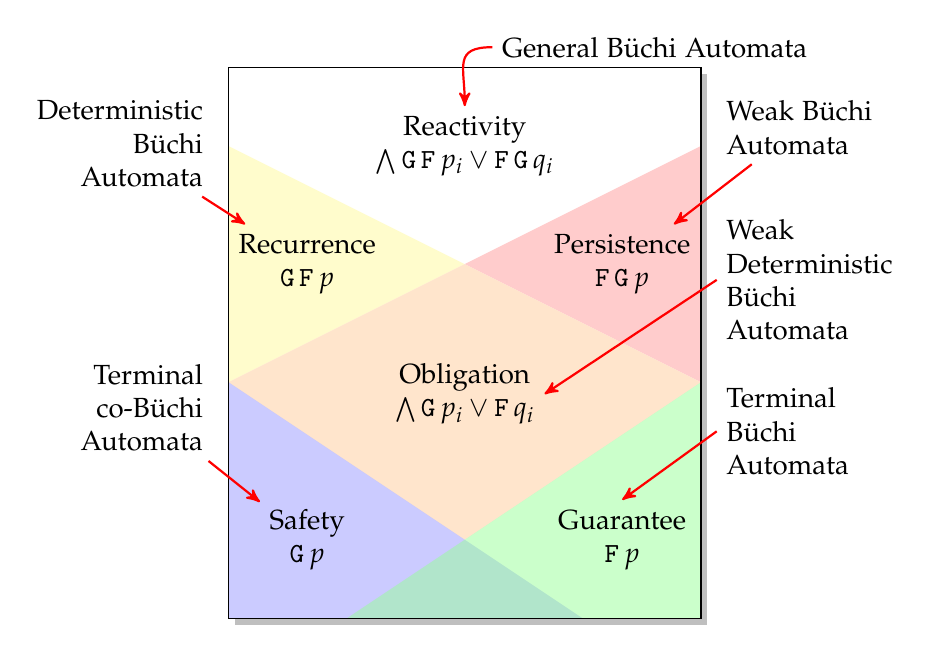
\begin{tikzpicture}
    \draw[drop shadow,fill=white] (0,0) rectangle (6,7);
    \path[fill=yellow!20] (0,6) -- (3,4.5) -- (0,3);
    \path[fill=red!20] (6,6) -- (3,4.5) -- (6,3);
    \path[fill=orange!20] (0,3) -- (3,4.5) -- (6,3) -- (3,1);
    \path[fill=blue!40,fill opacity=.5] (0,0) -- (0,3) -- (4.5,0);
    \path[fill=green!40,fill opacity=.5] (6,0) -- (1.5,0) -- (6,3);
    \draw (0,0) rectangle (6,7);

    \node[align=center] (rea) at (3,6)  {Reactivity\\ $\bigwedge\G\F p_i\lor \F\G q_i$};
    \node[align=center] (rec) at (1,4.5) {Recurrence\\ $\G\F p$};
    \node[align=center] (per) at (5,4.5) {Persistence\\ $\F\G p$};
    \node[align=center] (obl) at (3,2.85) {Obligation\\ $\bigwedge\G p_i\lor \F q_i$};
    \node[align=center] (saf) at (1,1) {Safety\\ $\G p$};
    \node[align=center] (gua) at (5,1) {Guarantee\\ $\F p$};

    \node[align=right,below left] (det) at (-.2,6.7) {Deterministic\\Büchi\\Automata};
    \node[align=left,below right](weak) at (6.2,6.7) {Weak Büchi\\Automata};
    \node[align=left,right](wdba) at (6.2,4.3) {Weak\\Deterministic\\Büchi\\Automata};
    \node[align=left,above right](ter) at (6.2,1.7) {Terminal\\Büchi\\Automata};
    \node[align=right,above left](occ) at (-.2,2) {Terminal\\co-Büchi\\Automata};

    \node[above right] (buc) at (3.35,7) {General Büchi Automata};

    \draw[annote] (rec) -- (det);
    \draw[annote] (per) -- (weak);
    \draw[annote] (obl.east) -- (wdba.west);
    \draw[annote] (gua.north) -- (ter.west);
    \draw[annote] (saf) -- (occ);
    \draw[annote] (rea.north) .. controls +(north:5mm) and +(west:5mm) .. (buc.west);
  \end{tikzpicture}
  \end{captionbeside}
\end{figure}

The hierarchy of linear temporal properties was introduced
by~\citet{manna.87.podc} and is illustrated on
Fig.~\ref{fig:hierarchy}.  In the case of the LTL subset of the
hierarchy, a first syntactic characterization of the classes was
presented by~\citet{chang.92.icalp}, but other presentations have been
done including negation~\citep{cerna.03.mfcs} and weak
until~\citep{schneider.01.lpar}.

The following grammar rules extend the aforementioned work slightly by
dealing with PSL operators.  These are the rules used by Spot to
decide upon construction to which class a formula belongs (see the
methods \texttt{is\_syntactic\_safety()},
\texttt{is\_syntactic\_guarantee()},
\texttt{is\_syntactic\_obligation()},
\texttt{is\_syntactic\_recurrence()}, and
\texttt{is\_syntactic\_persistence()} listed on
page~\pageref{property-methods}).

The symbols $\varphi_G$, $\varphi_S$, $\varphi_O$, $\varphi_P$,
$\varphi_R$ denote any formula belonging respectively to the
Guarantee, Safety, Obligation, Persistence, or Recurrence classes.
Additionally $\varphi_B$ denotes a finite LTL formula (the unnamed
class at the intersection of Safety and Guarantee formulas, at the
\textbf{b}ottom of Fig.~\ref{fig:hierarchy}).  $v$ denotes any
variable, $r$ any SERE, $r_F$ any bounded SERE (no loops), and $r_I$
any unbounded SERE.

\begin{align*}
  \varphi_B ::={}& \0\mid\1\mid v\mid\NOT\varphi_B\mid\varphi_B\AND\varphi_B
                   \mid(\varphi_B\OR\varphi_B)\mid\varphi_B\EQUIV\varphi_B
                   \mid\varphi_B\XOR\varphi_B\mid\varphi_B\IMPLIES\varphi_B
                   \mid\X\varphi_B\\
               \mid{}& \sere{r_F}\mid \nsere{r_F}\\
  \varphi_G ::={}& \varphi_B\mid \NOT\varphi_S\mid
                   \varphi_G\AND \varphi_G\mid (\varphi_G\OR \varphi_G)
                   \mid\varphi_S\IMPLIES\varphi_G\mid
                   \X\varphi_G \mid \F\varphi_G\mid
                   \varphi_G\U\varphi_G\mid \varphi_G\M\varphi_G\\
           \mid{}& \nsere{r}\mid
                   \sere{r}\Esuffix \varphi_G\mid
                   \sere{r_F}\Asuffix \varphi_G \\
  \varphi_S ::={}& \varphi_B\mid \NOT\varphi_G\mid
                   \varphi_S\AND \varphi_S\mid (\varphi_S\OR \varphi_S)
                   \mid\varphi_G\IMPLIES\varphi_S\mid
                   \X\varphi_S \mid \G\varphi_S\mid
                   \varphi_S\R\varphi_S\mid \varphi_S\W\varphi_S\\
           \mid{}& \sere{r}\mid
                   \sere{r_F}\Esuffix \varphi_S\mid
                   \sere{r}\Asuffix \varphi_S\\
  \varphi_O ::={}& \varphi_G \mid \varphi_S\mid \NOT\varphi_O\mid
                   \varphi_O\AND \varphi_O\mid (\varphi_O\OR \varphi_O)\mid
                   \varphi_O\EQUIV \varphi_O\mid \varphi_O\XOR \varphi_O\mid
                   \varphi_O\IMPLIES \varphi_O\\
           \mid{}& \X\varphi_O \mid
                   \varphi_O\U\varphi_G\mid\varphi_O\R\varphi_S \mid
                   \varphi_S\W\varphi_O\mid \varphi_G\M\varphi_O\\
           \mid{}& \sere{r} \mid \nsere{r}\mid
                   \sere{r_F}\Esuffix \varphi_O \mid \sere{r_I}\Esuffix \varphi_G\mid
                   \sere{r_F}\Asuffix \varphi_O\mid
                   \sere{r_I}\Asuffix \varphi_S\\
  \varphi_P ::={}& \varphi_O \mid \NOT\varphi_R\mid
                   \varphi_P\AND \varphi_P\mid (\varphi_P\OR \varphi_P)\mid
                   \varphi_P\EQUIV \varphi_P\mid \varphi_P\XOR \varphi_P\mid
                   \varphi_P\IMPLIES \varphi_P\\
           \mid{}& \X\varphi_P \mid \F\varphi_P \mid
                   \varphi_P\U\varphi_P\mid\varphi_P\R\varphi_S\mid
                   \varphi_S\W\varphi_P\mid\varphi_P\M\varphi_P\\
           \mid{}& \sere{r}\Esuffix \varphi_P\mid
                   \sere{r_F}\Asuffix \varphi_P\mid
                   \sere{r_I}\Asuffix \varphi_S\\
  \varphi_R ::={}& \varphi_O \mid \NOT\varphi_P\mid
                   \varphi_R\AND \varphi_R\mid (\varphi_R\OR \varphi_R)\mid
                   \varphi_R\EQUIV \varphi_R\mid \varphi_R\XOR \varphi_R\mid
                   \varphi_R\IMPLIES \varphi_R\\
           \mid{}& \X\varphi_R \mid \G\varphi_R \mid
                   \varphi_R\U\varphi_G\mid\varphi_R\R\varphi_R\mid
                   \varphi_R\W\varphi_R\mid\varphi_G\M\varphi_R\\
           \mid{}& \sere{r}\Asuffix \varphi_R\mid \sere{r_F}\Esuffix \varphi_R \mid \sere{r_I}\Esuffix \varphi_G\\
\end{align*}

It should be noted that a formula can belong to a class of the
temporal hierarchy even if it does not syntactically appears so.  For
instance the formula $(\G(q\OR \F\G p)\AND \G(r\OR \F\G\NOT p))\OR\G
q\OR \G r$ is not syntactically safe, yet it is a safety formula
equivalent to $\G q\OR \G r$.  Such a formula is usually said
\emph{pathologically safe}.

\chapter{Rewritings}

\section{Unabbreviations}\label{sec:unabbrev}

The `\verb=unabbreviate()=' function can apply the following rewriting
rules when passed a string denoting the list of rules to apply.  For
instance passing the string \texttt{"\^{}ei"} will rewrite all
occurrences of $\XOR$, $\EQUIV$ and $\IMPLIES$.

\[
\begin{array}{l@{\qquad}r@{\;}c@{\;}ll}
``\texttt{i}" & f\IMPLIES g &\equiv&  (\NOT f)\OR g\\
``\texttt{e}" & f\EQUIV g &\equiv&  (f\AND g)\OR ((\NOT g)\AND(\NOT f))\\
``\texttt{\^{}e}" & f\XOR g &\equiv&  (f\AND\NOT g)\OR (g\AND\NOT f)\\
``\texttt{\^{}}"\text{~without~}``\texttt{e}" & f\XOR g &\equiv&  \NOT(f\EQUIV g)\\
``\texttt{F}" & \F e&\equiv& e & \text{when $e$ is a pure eventuality}\\
``\texttt{F}" & \F f&\equiv& \1\U f\\
``\texttt{G}" & \G u&\equiv& u & \text{when $u$ is purely universal}\\
``\texttt{G}"\text{~without~}``\texttt{R}" & \G f&\equiv& \0\R f \\
``\texttt{GR}"\text{~without~}``\texttt{W}" & \G f&\equiv& f \W \0 \\
``\texttt{GRW}" & \G f&\equiv& \NOT\F\NOT f \\
``\texttt{M}" & f \M e&\equiv& \F(f\AND e) & \text{when $e$ is a pure eventuality} \\
``\texttt{M}" & f \M g&\equiv& g \U (g \AND f) \\
``\texttt{R}" & f \R u&\equiv& u & \text{when $u$ is purely universal} \\
``\texttt{R}"\text{~without~}``\texttt{W}" & f \R g&\equiv&  g\W (f \AND g)\\
``\texttt{RW}" & f \R g&\equiv&  g\U ((f \AND g) \OR \G g) \\
``\texttt{W}" & f \W u&\equiv& \G(f \OR u) & \text{when $u$ is purely universal} \\
``\texttt{W}"\text{~without~}``\texttt{R}" & f \W g&\equiv& g \R (g \OR f)\\
``\texttt{WR}" & f \W g&\equiv& f \U (g \OR \G f)\\
\end{array}
\]

Among all the possible rewritings (see Appendix~\ref{sec:ltl-equiv})
the default rules for $\R$, $\W$ and $\M$, those were chosen because
they are easier to translate in a tableau
construction~\cite[Fig.~11]{duret.11.vecos}.

Besides the `\verb=unabbreviate()=' function, there is also a class
`\verb=unabbreviator()= that implements the same functionality, but
maintains a cache of abbreviated subformulas.  This is preferable if
you plan to abbreviate many formulas sharing identical subformulas.

\section{LTL simplifier}

The LTL rewritings described in the next three sections are all
implemented in the `\verb|tl_simplifier|' class defined in
\texttt{spot/tl/simplify.hh}.  This class implements several
caches in order to quickly rewrite formulas that have already been
rewritten previously.  For this reason, it is suggested that you reuse
your instance of `\verb|tl_simplifier|' as much as possible.  If you
write an algorithm that will simplify LTL formulas, we suggest you
accept an optional `\verb|tl_simplifier|' argument, so that you can
benefit from an existing instance.

The `\verb|tl_simplifier|' takes an optional
`\verb|tl_simplifier_options|' argument, making it possible to tune
the various rewritings that can be performed by this class.  These
options cannot be changed afterwards (because changing these options
would invalidate the results stored in the caches).

\section{Negative normal form}\label{sec:nnf}

This is implemented by the `\verb|tl_simplifier::negative_normal_form|`
method.

A formula in negative normal form can only have negation
operators ($\NOT$) in front of atomic properties, and does not use any
of the $\XOR$, $\IMPLIES$ and $\EQUIV$ operators.  The following
rewriting arrange any PSL formula into negative normal form.

\begin{align*}
  \NOT\X f & \equiv \X\NOT f &
  \NOT(f \U g) & \equiv (\NOT f) \R (\NOT g) &
  \NOT(f \AND g)&\equiv (\NOT f) \OR (\NOT g)
  \\
  \NOT\F f & \equiv \G\NOT f &
  \NOT(f \R g) & \equiv (\NOT f) \U (\NOT g) &
  \NOT(f \OR g)&\equiv (\NOT f)\AND (\NOT g)
  \\
  \NOT\G f & \equiv \F\NOT f &
  \NOT(f \W g) & \equiv (\NOT f) \M (\NOT g) &
  \NOT(\sere{r} \Asuffix f) &\equiv \sere{r} \Esuffix \NOT f
  \\
  \NOT(\sere{r})&\equiv \nsere{r}&
  \NOT(f \M g) & \equiv (\NOT f) \W (\NOT g)&
  \NOT(\sere{r} \Esuffix f) &\equiv \sere{r} \Asuffix \NOT f
\end{align*}
\noindent Recall that the negated weak closure $\nsere{r}$ is actually
implemented as a specific operator, so it is not actually prefixed by the
$\NOT$ operator.
\begin{align*}
  f \XOR g & \equiv ((\NOT f)\AND g)\OR(f\AND\NOT g) &
  \NOT(f \XOR g) & \equiv ((\NOT f)\AND(\NOT g))\OR(f\AND g) &
  \NOT(f \AND g) & \equiv (\NOT f)\OR(\NOT g) \\
  f \EQUIV g & \equiv ((\NOT f)\AND(\NOT g))\OR(f\AND g) &
  \NOT(f \EQUIV g) & \equiv ((\NOT f)\AND g)\OR(f\AND\NOT g) &
  \NOT(f \OR g) & \equiv (\NOT f)\AND(\NOT g) \\
  f \IMPLIES g & \equiv (\NOT f) \AND g &
  \NOT(f \IMPLIES g) & \equiv f \AND \NOT g
\end{align*}

Note that the above rules include the ``unabbreviation'' of operators
``$\EQUIV$'', ``$\IMPLIES$'', and ``$\XOR$'', correspondings to the
rules \texttt{"ei\^"} of function `\verb=unabbreviate()= as described
in Section~\ref{sec:unabbrev}.  Therefore it is never necessary to
apply these abbreviations before or after
`\verb|tl_simplifier::negative_normal_form|`.

If the option `\verb|nenoform_stop_on_boolean|' is set, the above
recursive rewritings are not applied to Boolean subformulas.  For
instance calling `\verb|tl_simplifier::negative_normal_form|` on
$\NOT\F\G(a \XOR b)$ will produce $\G\F(((\NOT a)\AND(\NOT
b))\OR(a\AND b))$ if `\verb|nenoform_stop_on_boolean|' is unset, while
it will produce $\G\F(\NOT(a \XOR b))$ if
`\verb|nenoform_stop_on_boolean|' is set.

\section{Simplifications}

The `\verb|tl_simplifier::simplify|' method performs several kinds of
simplifications, depending on which `\verb|tl_simplifier_options|'
was set.

The goals in most of these simplification are to:
\begin{itemize}
\item remove useless terms and operator.
\item move the $\X$ operators to the front of the formula (e.g., $\X\G
  f$ is better than the equivalent $\G\X f$).  This is because LTL
  translators will usually want to rewrite LTL formulas in
  a kind of disjunctive form: $\displaystyle\bigvee_i
  \left(\beta_i\land\X\psi_i\right)$ where $\beta_i$s are Boolean
  formulas and $\psi_i$s are LTL formulas.  Moving $\X$ to the
  front therefore simplifies the translation.
\item move the $\F$ operators to the front of the formula (e.g., $\F(f
  \OR g)$ is better than the equivalent $(\F f)\OR (\F g)$), but not
  before $\X$ ($\X\F f$ is better than $\F\X f$).  Because $\F f$
  incurs some indeterminism, it is best to factorize these terms to
  limit the sources of indeterminism.
\end{itemize}

Rewritings defined with $\equivEU$ are applied only when
\verb|tl_simplifier_options::favor_event_univ|' is \texttt{true}:
they try to lift subformulas that are both eventual and universal
\emph{higher} in the syntax tree.  Conversely, rules defined with $\equivNeu$
are applied only when \verb|favor_event_univ|' is \texttt{false}: they
try to \textit{lower} subformulas that are both eventual and universal.

\subsection{Basic Simplifications}\label{sec:basic-simp}

These simplifications are enabled with
\verb|tl_simplifier_options::reduce_basics|'.  A couple of them may
enlarge the size of the formula: they are denoted using $\equiV$
instead of $\equiv$, and they can be disabled by setting the
\verb|tl_simplifier_options::reduce_size_strictly|' option to
\texttt{true}.

\subsubsection{Basic Simplifications for Temporal Operators}
\label{sec:basic-simp-ltl}

The following are simplification rules for unary operators (applied
from left to right, as usual):
\begin{align*}
  \X\F\G f                                                    & \equiv \F\G f & \F(f\U g)        & \equiv \F g             & \G(f \R g)      & \equiv \G g             \\
  \X\G\F f                                                    & \equiv \G\F f & \F(f\M g)        & \equiv \F (f\AND g)     & \G(f \W g)      & \equiv \G(f\OR g)       \\
\F\X f                                                        & \equiv \X\F f & \F\G(f\AND \X g) & \equiv \F\G(f\AND g)    & \G\F(f\OR \X g) & \equiv \G\F(f\OR g)     \\
\G\X f                                                        & \equiv \X\G f & \F\G(f\AND \G g) & \equiv \F\G(f\AND g)    & \G\F(f\OR \F g) & \equiv \G\F(f\OR g)     \\
                                                              &               & \F\G(f\OR\G g)   & \equiv \F(\G f\OR\G g)  & \G\F(f\AND\F g) & \equiv \G(\F f\AND\F g) \\
                                                              &               & \F\G(f\AND\F g)  & \equiV \F\G f\AND\G\F g & \G\F(f\AND\G g) & \equiV \G\F f\AND\F\G g \\
                                                              &               & \F\G(f\OR\F g)  & \equivEU \F\G f\OR\G\F g & \G\F(f\OR\G g) & \equivEU \G\F f\OR\F\G g
\end{align*}
\begin{align*}
  \G(f_1\OR\ldots\OR f_n \OR \G\F(g_1)\OR\ldots\OR \G\F(g_m)) & \equiv \G(f_1\OR\ldots\OR f_n)\OR \G\F(g_1\OR\ldots\OR g_m)
\end{align*}

% Note that the latter three rewriting rules for $\G$ have no dual:
% rewriting $\F(f \AND \G\F g)$ to $\F(f) \AND \G\F(g)$ (as suggested
% by~\citet{somenzi.00.cav}) goes against our goal of moving the $\F$
% operator in front of the formula.  Conceptually, it is also easier to
% understand $\F(f \AND \G\F g)$: has long as $f$ has not been verified,
% there is no need to worry about the $\G\F g$ term.

Here are the basic rewriting rules for binary operators (excluding
$\OR$ and $\AND$ which are considered in Spot as $n$-ary operators).
$b$ denotes any Boolean formula.

\begin{align*}
  \1 \U f             & \equiv \F f            & f \W \0             & \equiv \G f            \\
  f \M \1             & \equiv \F f            & \0 \R f             & \equiv \G f            \\
  (\X f)\U (\X g)     & \equiv \X(f\U g)       & (\X f)\W(\X g)      & \equiv \X(f\W g)       \\
  (\X f)\M (\X g)     & \equiv \X(f\M g)       & (\X f)\R(\X g)      & \equiv \X(f\R g)       \\
  (\X f)\U b          & \equiV b\OR \X(b\M f)  & (\X f)\W b          & \equiV b\OR \X(f\R b)  \\
  (\X f)\M b          & \equiV b\AND \X(b\U f) & (\X f)\R b          & \equiV b\AND \X(f\W b) \\
  f \U(\G f)          & \equiv \G f            & f \W(\G f)          & \equiv \G f            \\
  f \M(\F f)          & \equiv \F f            & f \R(\F f)          & \equiv \F f            \\
  f \U (g \OR \G(f))  & \equiv f\W g           & f \W (g \OR \G(f))  & \equiv f\W g           \\
  f \M (g \AND \F(f)) & \equiv f\M g           & f \R (g \AND \F(f)) & \equiv f\M g           \\
  f \U (g \AND f)     & \equiv g\M f           & f \W (g \AND f)     & \equiv g\R f           \\
  f \M (g \OR f)      & \equiv g\U f           & f \R (g \OR f)      & \equiv g\W f
\end{align*}

Here are the basic rewriting rules for $n$-ary operators ($\AND$ and
$\OR$):
\begin{align*}
  (\F\G f) \AND(\F\G g) &\equiv \F\G(f\AND g)     &
  (\G\F f) \OR (\G\F g) &\equiv \G\F(f\OR g)      \\
  (\X f) \AND(\X g)     &\equiv \X(f\AND g)       &
  (\X f) \OR (\X g)     &\equiv \X(f\OR g)        \\
  (\X f) \AND(\F\G g)   &\equivNeu \X(f\AND \F\G g)  &
  (\X f) \OR (\G\F g)   &\equivNeu \X(f\OR \G\F g)  \\
  (\G f) \AND(\G g)     &\equivNeu \G(f\AND g)       &
  (\F f) \OR (\F g)     &\equivNeu \F(f\OR g)        \\
  (f_1 \U f_2)\AND (f_3 \U f_2)&\equiv (f_1\AND f_3)\U f_2&
  (f_1 \U f_2)\OR  (f_1 \U f_3)&\equiv f_1\U (f_2\OR f_3) \\
  (f_1 \U f_2)\AND (f_3 \W f_2)&\equiv (f_1\AND f_3)\U f_2&
  (f_1 \U f_2)\OR  (f_1 \W f_3)&\equiv f_1\W (f_2\OR f_3) \\
  (f_1 \W f_2)\AND (f_3 \W f_2)&\equiv (f_1\AND f_3)\W f_2&
  (f_1 \W f_2)\OR  (f_1 \W f_3)&\equiv f_1\W (f_2\OR f_3) \\
  (f_1 \R f_2)\AND (f_1 \R f_3)&\equiv f_1\R (f_2\AND f_3)&
  (f_1 \R f_2)\OR  (f_3 \R f_2)&\equiv (f_1\OR f_3) \R f_2\\
  (f_1 \R f_2)\AND (f_1 \M f_3)&\equiv f_1\M (f_2\AND f_3)&
  (f_1 \R f_2)\OR  (f_3 \M f_2)&\equiv (f_1\OR f_3) \R f_3\\
  (f_1 \M f_2)\AND (f_1 \M f_3)&\equiv f_1\M (f_2\AND f_3)&
  (f_1 \M f_2)\OR  (f_3 \M f_2)&\equiv (f_1\OR f_3) \M f_3\\
  (\F g)\AND (f \U g)&\equiv f\U g &
  (\G f)\OR  (f \U g)&\equiv f\W g \\
  (\F g)\AND (f \W g)&\equiv f\U g &
  (\G f)\OR  (f \W g)&\equiv f\W g \\
  (\F f)\AND (f \R g)&\equiv f\M g &
  (\G g)\OR  (f \R g)&\equiv f\R g \\
  (\F f)\AND (f \M g)&\equiv f\M g &
  (\G g)\OR  (f \M g)&\equiv f\R g \\
  f \AND ((\X f) \W g) &\equiv g \R f &
  f \OR ((\X f) \R g) &\equiv g \W f \\
  f \AND ((\X f) \U g) &\equiv g \M f &
  f \OR ((\X f) \M g) &\equiv g \U f \\
  f \AND (g \OR \X(g \R f)) &\equiv g \R f &
  f \OR (g \AND \X(g \W f)) &\equiv g \W f \\
  f \AND (g \OR \X(g \M f)) &\equiv g \M f &
  f \OR (g \AND \X(g \U f)) &\equiv g \U f \\
\end{align*}
The above rules are applied even if more terms are presents in the
operator's arguments.  For instance $\F\G(a)\AND \G(b) \AND \F\G(c) \AND
\X(d)$ will be rewritten as $\X(d \AND \F\G(a\AND c))\AND \G(b)$.

The following more complicated rules are generalizations of $f\AND
\X\G f\equiv \G f$ and $f\OR \X\F f\equiv \F f$:
\begin{align*}
  f\AND \X(\G(f\AND g\AND \ldots)\AND h\AND \ldots) &\equiv \G(f) \AND \X(\G(g\AND \ldots)\AND h\AND \ldots) \\
  f\OR \X(\F(f)\OR h\OR \ldots) &\equiv \F(f) \OR \X(h\OR \ldots)
\end{align*}
The latter rule for $f\OR \X(\F(f)\OR h\ldots)$ is only applied if all
$\F$-formulas can be removed from the argument of $\X$ with the
rewriting.  For instance $a \OR b \OR c\OR \X(\F(a\OR b)\OR \F(c)\OR \G d)$
will be rewritten to $\F(a \OR b \OR c) \OR \X\G d$ but
$b \OR c\OR \X(\F(a\OR b)\OR \F(c)\OR \G d)$ will only become
$b \OR c\OR \X(\F(a\OR b\OR c)\OR \G d)$.

Finally the following rule is applied only when no other terms are present
in the OR arguments:
\begin{align*}
  \F(f_1) \OR \ldots \OR \F(f_n) \OR \G\F(g)
   &\equivNeu \F(f_1\OR \ldots \OR f_n \OR \G\F(g)) \\
\end{align*}

\subsubsection{Basic Simplifications for SERE Operators}

\spottodo[inline]{The following rules, mostly taken
  from~\citet{cimatti.08.tcad} are not complete yet.  We only show
  those that are implemented.}

The following simplification rules are used for the $n$-ary operators
$\ANDALT$, $\AND$, and $\OR$.  The patterns are of course commutative.
$b$ or $b_i$ denote any Boolean formula while $r$ or $r_i$ denote any
SERE.

\begin{align*}
  b \ANDALT r\STAR{\mvar{i}..\mvar{j}} &\equiv
  \begin{cases}
    b \ANDALT r &\text{if~} i\le 1\le j\\
    \0 &\text{else}\\
  \end{cases} &
  b \AND r &\equiV
  \begin{cases}
    b \OR \mathtt{\{}b\FUSION r\mathtt{\}}&\text{if~} \varepsilon\VDash r_i\\
    b\FUSION r&\text{if~} \varepsilon\not\VDash r_i\\
  \end{cases} \\
  b \ANDALT \sere{r_1 \FUSION \ldots \FUSION r_n} &\equiv b \ANDALT r_1 \ANDALT \ldots \ANDALT r_n \\
  b \ANDALT \sere{r_1 \CONCAT \ldots \CONCAT r_n} &\equiv
  \begin{cases}
    b \ANDALT r_i & \text{if~}\exists!i,\,\varepsilon\not\VDash r_i\\
    b \ANDALT (r_1 \OR \ldots \OR r_n) & \text{if~}\forall i,\, \varepsilon\VDash r_i\\
    \0 &\text{else}\\
  \end{cases}\\
  \sere{b_1\CONCAT r_1}\ANDALT\sere{b_2\CONCAT r_2} &\equiv \sere{b_1\ANDALT b_2}\CONCAT\sere{r_1\ANDALT r_2} &
  \sere{r_1\CONCAT b_1}\ANDALT\sere{r_2\CONCAT b_2} &\equiv \sere{r_1\ANDALT r_2}\CONCAT\sere{b_1\ANDALT b_2} \\
  \sere{b_1\FUSION r_1}\ANDALT\sere{b_2\FUSION r_2} &\equiv \sere{b_1\ANDALT b_2}\FUSION\sere{r_1\ANDALT r_2} &
  \sere{r_1\FUSION b_1}\ANDALT\sere{r_2\FUSION b_2} &\equiv \sere{r_1\ANDALT r_2}\FUSION\sere{b_1\ANDALT b_2} \\
  \sere{b_1\CONCAT r_1}\AND \sere{b_2\CONCAT r_2} &\equiv \sere{b_1\ANDALT b_2}\CONCAT\sere{r_1\AND r_2} \\
  \sere{b_1\FUSION r_1}\AND \sere{b_2\FUSION r_2} &\equiv \sere{b_1\ANDALT b_2}\FUSION\sere{r_1\AND r_2} \mathrlap{\quad\text{if~}\varepsilon\nVDash r_1\land\varepsilon\nVDash r_2}
\end{align*}
\begin{align*}
  \FIRSTMATCH\code(b\STAR{\mvar{i}..\mvar{j}}\code) &\equiv b\STAR{\mvar{i}} \\
  \FIRSTMATCH\code(r\STAR{\mvar{i}..\mvar{j}}\code) &\equiv \FIRSTMATCH\code(r\STAR{\mvar{i}}\code) \\
  \FIRSTMATCH\code(r\FSTAR{\mvar{i}..\mvar{j}}\code) &\equiv \FIRSTMATCH\code(r\FSTAR{\mvar{i}}\code) \\
  \FIRSTMATCH\code(r_1\CONCAT{}r_2\STAR{\mvar{i}..\mvar{j}}\code) &\equiv \FIRSTMATCH\code(r_1\CONCAT{}r_2\STAR{\mvar{i}}\code) \\
  \FIRSTMATCH\code(r_1\CONCAT{}r_2\FSTAR{\mvar{i}..\mvar{j}}\code) &\equiv \FIRSTMATCH\code(r_1\CONCAT{}r_2\FSTAR{\mvar{i}}\code) \\
  \FIRSTMATCH\code(r_1\FUSION{}r_2\STAR{\mvar{i}..\mvar{j}}\code) &\equiv \FIRSTMATCH\code(r_1\FUSION{}r_2\STAR{\mvar{\max(i,1)}}\code) \\
  \FIRSTMATCH\code(r_1\FUSION{}r_2\FSTAR{\mvar{i}..\mvar{j}}\code) &\equiv \FIRSTMATCH\code(r_1\FUSION{}r_2\FSTAR{\mvar{i}}\code) \\
  \FIRSTMATCH\code(b\CONCAT{}r\code) &\equiv b\CONCAT\FIRSTMATCH\code(r\code) \\
  \FIRSTMATCH\code(b\STAR{\mvar{i}..\mvar{j}}\CONCAT{}r\code) &\equiv b\STAR{\mvar{i}}\CONCAT\FIRSTMATCH\code(b\STAR{0..\mvar{j-i}}\CONCAT r\code) \\
  \FIRSTMATCH\code(b\STAR{\mvar{i}..\mvar{j}}\FUSION{}r\code) &\equiv b\STAR{\mvar{i-1}}\CONCAT\FIRSTMATCH\code(b\STAR{1..\mvar{j-i+1}}\FUSION r\code)\quad\text{if~}i>1\\
  \FIRSTMATCH\code(r_1\CONCAT{}r_2\code) &\equiv\FIRSTMATCH\code(r_1\code)\quad\text{if~} \varepsilon\VDash r_2\\
  \FIRSTMATCH\code(\FIRSTMATCH\code(r_1\code)\CONCAT{}r_2\code) &\equiv\FIRSTMATCH\code(r_1\code)\CONCAT\FIRSTMATCH\code(r_2\code)\\
  \FIRSTMATCH\code(\FIRSTMATCH\code(r_1\code)\FUSION{}r_2\code) &\equiv\FIRSTMATCH\code(r_1\code)\FUSION\FIRSTMATCH\code(\1\FUSION{}r_2\code)
\end{align*}

Starred subformulas are rewritten in Star Normal
Form~\cite{bruggeman.96.tcs} with:
\[r\STAR{} \equiv r^\circ\STAR{} \]
where $r^\circ$ is recursively defined as follows:
\begin{align*}
  r^\circ &= r\text{~if~} \varepsilon\not\VDash r \\
  \eword^\circ &= \0 &
  (r_1\CONCAT r_2)^\circ &= r_1^\circ\OR r_2^\circ \text{~if~} \varepsilon\VDash r_1\text{~and~}\varepsilon\VDash r_2\\
  r\STAR{\mvar{i}..\mvar{j}}^\circ &= r^\circ \text{~if~} i=0 \text{~or~} \varepsilon\VDash r&
  (r_1\AND r_2)^\circ &= r_1^\circ\OR r_2^\circ \text{~if~} \varepsilon\VDash r_1\text{~and~}\varepsilon\VDash r_2\\
  (r_1\OR r_2)^\circ &= r_1^\circ \OR r_2^\circ &
  (r_1\ANDALT r_2)^\circ &= r_1 \ANDALT r_2
\end{align*}

Note: the original SNF definition~\cite{bruggeman.96.tcs} does not
include \samp{$\AND$} and \samp{$\ANDALT$} operators, and it
guarantees that $\forall r,\,\varepsilon\not\VDash r^\circ$ because
$r^\circ$ is stripping all the stars and empty words that occur in
$r$.  For instance $\sere{a\STAR{}\CONCAT
  b\STAR{}\CONCAT\sere{\eword\OR c}}^\circ\STAR{} = \sere{a\OR b\OR
  c}\STAR{}$.  Our extended definition still respects this property in
presence of \samp{$\AND$} operators, but unfortunately not when the
\samp{$\ANDALT$} operator is used.

We extend the above definition to bounded repetitions with:
\begin{align*}
  r\STAR{\mvar{i}..\mvar{j}} & \equiv r^\square\STAR{0..\mvar{j}}\quad\text{if}\quad\varepsilon\VDash r\STAR{\mvar{i}..\mvar{j}},\,\varepsilon\not\VDash r^\square,\,\text{~and~}j>1\\
  r\STAR{\mvar{i}..\mvar{j}} & \equiv r^\square\STAR{1..\mvar{j}}\quad\text{if}\quad\varepsilon\VDash r\STAR{\mvar{i}..\mvar{j}},\,\varepsilon\VDash r^\square\,\text{~and~}j>1\\
  r\STAR{\mvar{i}..\mvar{j}} & \equiv r\phantom{^\square\STAR{1..\mvar{j}}}\quad\text{if}\quad\varepsilon\VDash r\text{~and~}\mvar{j}=1
\end{align*}
where $r^\square$ is recursively defined as follows:
\begin{align*}
  r^\square &= r\text{~if~} \varepsilon\not\VDash r \\
  \eword^\square &= \0 &
  (r_1\CONCAT r_2)^\square &= r_1\CONCAT r_2\\
  r\STAR{\mvar{i}..\mvar{j}}^\square &= r^\square\STAR{\mvar{\max(1,i)}..\mvar{j}} \text{~if~} i=0 \text{~or~} \varepsilon\VDash r &
  (r_1\AND r_2)^\square &= r_1^\square\OR r_2^\square \text{~if~} \varepsilon\VDash r_1\text{~and~}\varepsilon\VDash r_2\\
  (r_1\OR r_2)^\square &= r_1^\square \OR r_2^\square &
  (r_1\ANDALT r_2)^\square &= r_1 \ANDALT r_2
\end{align*}
The differences between $^\square$ and $^\circ$ are in the handling
of $r\STAR{\mvar{i}..\mvar{j}}$ and in the handling of $r_1\CONCAT r_2$.

% Indeed $(c\STAR{}\OR\1)\STAR{0..1}$ is not equivalent to
% $(c\STAR{}\OR\1)^\circ\STAR{0..1}\equiv(c\OR\1)\STAR{0..1}\equiv
% 1\STAR{0..1}$ but to
% $(c\STAR{}\OR\1)^\square\STAR{0..1}\equiv(c\PLUS{}\OR\1)\STAR{0..1}$.

% Similarly $(a\STAR{}\CONCAT b\STAR{})\STAR{0..1})$ is definitely not
% equal to $(a\PLUS{}\OR b\PLUS{})\STAR{0..1}).


\subsubsection{Basic Simplifications SERE-LTL Binding Operators}

The following rewritings are applied to the operators $\Asuffix$ and
$\Esuffix$.  They assume that $b$, denote a Boolean formula.

As noted at the beginning for section~\ref{sec:basic-simp}, rewritings
denoted with $\equiV$ can be disabled by setting the
\verb|tl_simplifier_options::reduce_size_strictly|' option to
\texttt{true}.

\begin{align*}
  \sere{\STAR{}}\Asuffix f &\equiv \G f\\
  \sere{b\STAR{}}\Asuffix f &\equiv f \W \NOT b\\
  \sere{b\PLUS{}}\Asuffix f &\equiv f \W \NOT b\\
  \sere{r\STAR{0..\mvar{j}}}\Asuffix f &\equiv \sere{r\STAR{1..\mvar{j}}}\Asuffix f \\
  \sere{r\STAR{\mvar{i}..\mvar{j}}}\Asuffix f &\equiV
    \sere{r}\Asuffix \X(
    \sere{r}\Asuffix \X(\ldots
    \Asuffix\X(r\STAR{\mvar{1}..\mvar{j-i+1}})))
    \text{~if~}i\ge 1\text{~and~}\varepsilon\not\VDash r\\
  \sere{r\CONCAT \STAR{}}\Asuffix f &\equiv \sere{r}\Asuffix \G f\\
  \sere{r\CONCAT b\STAR{}}\Asuffix f &\equiV \sere{r}\Asuffix (f\AND \X(f \W \NOT b)) \text{~if~}\varepsilon\not\VDash r\\
  \sere{\STAR{}\CONCAT r}\Asuffix f &\equiV \G(\sere{r}\Asuffix f)\\
  \sere{b\STAR{}\CONCAT r}\Asuffix f &\equiV (\NOT b)\R(\sere{r}\Asuffix f) \text{~if~}\varepsilon\not\VDash r\\
  \sere{r_1\CONCAT r_2}\Asuffix f &\equiV \sere{r_1}\Asuffix\X(\sere{r_2}\Asuffix f)\text{~if~}\varepsilon\not\VDash r_1\text{~and~}\varepsilon\not\VDash r_2\\
  \sere{r_1\FUSION r_2}\Asuffix f &\equiV \sere{r_1}\Asuffix(\sere{r_2}\Asuffix f)\\
  \sere{r_1\OR r_2}\Asuffix f &\equiV (\sere{r_1}\Asuffix f)\AND(\sere{r_2}\Asuffix f)\\
  \sere{\STAR{}}\Esuffix f &\equiv \F f\\
  \sere{b\STAR{}}\Esuffix f &\equiv f \M b\\
  \sere{b\PLUS{}}\Esuffix f &\equiv f \M b\\
  \sere{r\STAR{0..\mvar{j}}}\Esuffix f &\equiv \sere{r\STAR{1..\mvar{j}}}\Esuffix f \\
  \sere{r\STAR{\mvar{i}..\mvar{j}}}\Esuffix f &\equiV
    \sere{r}\Esuffix \X(
    \sere{r}\Esuffix \X(\ldots
    \Esuffix\X(r\STAR{\mvar{1}..\mvar{j-i+1}})))
    \text{~if~}i\ge 1\text{~and~}\varepsilon\not\VDash r\\
  \sere{r\CONCAT \STAR{}}\Esuffix f &\equiv \sere{r}\Esuffix \F f\\
  \sere{r\CONCAT b\STAR{}}\Esuffix f &\equiV \sere{r}\Esuffix (f\OR \X(f \M b)) \text{~if~}\varepsilon\not\VDash r\\
  \sere{\STAR{}\CONCAT r}\Esuffix f &\equiV \F(\sere{r}\Esuffix f)\\
  \sere{b\STAR{}\CONCAT r}\Esuffix f &\equiV b\U(\sere{r}\Esuffix f) \text{~if~}\varepsilon\not\VDash r\\
  \sere{r_1\CONCAT r_2}\Esuffix f &\equiV \sere{r_1}\Esuffix\X(\sere{r_2}\Esuffix f)\text{~if~}\varepsilon\not\VDash r_1\text{~and~}\varepsilon\not\VDash r_2\\
  \sere{r_1\FUSION r_2}\Esuffix f &\equiV \sere{r_1}\Esuffix(\sere{r_2}\Esuffix f)\\
  \sere{r_1\OR r_2}\Esuffix f &\equiV (\sere{r_1}\Esuffix f)\OR(\sere{r_2}\Esuffix f)
\end{align*}

Here are the basic rewritings for the weak closure and its negation:
\begin{align*}
  \sere{r\STAR{}}&\equiv \sere{r}&
  \nsere{r\STAR{}}&\equiv \nsere{r}\\
  \sere{r;\1}&\equiv \sere{r} \quad\text{if~}\varepsilon\not\VDash r&
  \nsere{r;\1}&\equiv \nsere{r} \quad\text{if~}\varepsilon\not\VDash r\\
  \sere{r;\1}&\equiv \1 \quad\text{if~}\varepsilon\VDash r&
  \nsere{r;\1}&\equiv \0 \quad\text{if~}\varepsilon\VDash r\\
  \sere{r_1;r_2}&\equiv \sere{r_1}\phantom{{}\OR\sere{r_2}}\quad\text{if~}\varepsilon\not\VDash r_1\land\varepsilon\VDash r_2&
  \nsere{r_1;r_2}&\equiv \nsere{r_1}\phantom{{}\AND\nsere{r_2}}\quad\text{if~}\varepsilon\not\VDash r_1\land\varepsilon\VDash r_2\\
  \sere{r_1;r_2}&\equiv \sere{r_1}\OR\sere{r_2}\quad\text{if~}\varepsilon\VDash r_1\land\varepsilon\VDash r_2&
  \nsere{r_1;r_2}&\equiv \nsere{r_1}\AND\nsere{r_2}\quad\text{if~}\varepsilon\VDash r_1\land\varepsilon\VDash r_2\\
  \sere{b;r}&\equiV b\AND\X\sere{r}&
  \nsere{b;r}&\equiV (\NOT b)\OR\X\nsere{r}\\
% These two would be correct only if $r$ is satisfiable.
%  \sere{b\STAR{};r}&\equiv b\W\sere{r}&
%  \nsere{b\STAR{};r}&\equiv (\NOT b)\M\nsere{r}\\
  \sere{b\STAR{\mvar{i}..\mvar{j}};r}&\equiV \underbrace{b\AND \X(b\ldots}_{\mathclap{i\text{~occurences of~}b}}\AND\X\sere{b\STAR{\mvar{0}..\mvar{j-i}}\CONCAT r})&
  \nsere{b\STAR{\mvar{i}..\mvar{j}};r}&\equiV \underbrace{(\NOT b)\OR \X((\NOT b)\ldots}_{\mathclap{i\text{~occurences of~}\NOT b}}\OR\X\nsere{b\STAR{\mvar{0}..\mvar{j-i}}\CONCAT r}) \\
  \sere{b\STAR{\mvar{i}..\mvar{j}}}&\equiV \underbrace{b\AND \X(b\AND \X(\ldots b))}_{i\text{~occurences of~}b}&
  \nsere{b\STAR{\mvar{i}..\mvar{j}}}&\equiV \underbrace{(\NOT b)\OR \X((\NOT b)\OR \X(\ldots(\NOT b)))}_{i\text{~occurences of~}\NOT b}\\
  \sere{r_1\OR r_2}&\equiV\sere{r_1}\OR\sere{r_2} &
  \nsere{r_1\OR r_2}&\equiV\nsere{r_1}\AND\nsere{r_2}
\end{align*}

\subsection{Simplifications for Eventual and Universal Formulas}
\label{sec:eventunivrew}

The class of \textit{pure eventuality} and \textit{purely universal}
formulas are described in section~\ref{sec:eventuniv}.

In the following rewritings, we use the following
notation to distinguish the class of subformulas:

\begin{center}
\begin{tabular}{rl}
\toprule
$f,\,f_i,\,g,\,g_i$ & any PSL formula                                  \\
$e,\,e_i$           & a pure eventuality                               \\
$u,\,u_i$           & a purely universal formula                       \\
$q,\,q_i$           & a pure eventuality that is also purely universal \\
\bottomrule
\end{tabular}
\end{center}

\begin{align*}
  \F e        & \equiv e             & f \U e         & \equiv e                & e \M g        & \equiv e\AND g          & u_1 \M u_2 & \equiV (\F u_1) \AND u_2 \\
  \F(u)\OR q  & \equivNeu \F(u\OR q) & f \U (g\OR e)  & \equivEU (f \U g)\OR e  & f\M (g\AND u) & \equivEU (f \M g)\AND u & q \U\X f   & \equiv \X(q \U f)        \\
              &                      & f \U (g\AND q) & \equivEU (f \U g)\AND q & (f\AND q)\M g & \equivEU (f \M g)\AND q                                         \\
  \G u        & \equiv u             & u \W g         & \equiv u\OR g           & f \R u        & \equiv u                & e_1 \W e_2 & \equiV (\G e_1) \OR e_2  \\
  \G(e)\AND q & \equiv \G(e\AND q)   & f \W (g\OR e)  & \equivEU (f \W g)\OR e  & f\R (g\AND u) & \equivEU (f \R g)\AND u & q \R\X f   & \equiv \X(q \R f)        \\
  \X q        & \equiv q             & q \AND \X f    & \equivNeu \X(q \AND f)  & q\OR \X f     & \equivNeu \X(q \OR f)                                           \\
              &                      & \X(q \AND f)   & \equivEU q \AND \X f    & \X(q \OR f)   & \equivEU q\OR \X f                                              \\
\end{align*}

\begin{align*}
  \G(f_1\AND\ldots\AND f_n \AND \X e_1 \AND \ldots \AND \X e_p)&\equiv \G(f_1\AND\ldots\AND f_n \AND e_1 \AND \ldots \AND e_p) \\
  \G(f_1\AND\ldots\AND f_n \AND \F (g_1 \AND \ldots \AND g_p \AND \X e_1 \AND \ldots \AND \X e_m))&\equiv \G(f_1\AND\ldots\AND f_n \AND \F(g_1 \AND \ldots \AND g_p) \AND e_1 \AND \ldots \AND e_m) \\
  \F(f_1\OR\ldots\OR f_n \OR \X u_1 \OR \ldots \OR \X u_p)&\equiv \F(f_1\OR\ldots\OR f_n \OR u_1 \OR \ldots \OR u_p) \\
  \F(f_1\OR\ldots\OR f_n \OR \G (g_1 \OR \ldots \OR g_p \OR \X u_1 \OR \ldots \OR \X u_m))&\equiv \F(f_1\OR\ldots\AND f_n \OR \G(g_1 \OR \ldots \OR g_p) \OR u_1 \OR \ldots \OR u_m) \\
  \G(f_1\OR\ldots\OR f_n \OR q_1 \OR \ldots \OR q_p)&\equiv \G(f_1\OR\ldots\OR f_n)\OR q_1 \OR \ldots \OR q_p \\
  \F(f_1\AND\ldots\AND f_n \AND q_1 \AND \ldots \AND q_p)&\equivEU \F(f_1\AND\ldots\AND f_n)\AND q_1 \AND \ldots \AND q_p \\
  \G(f_1\AND\ldots\AND f_n \AND q_1 \AND \ldots \AND q_p)&\equivEU \G(f_1\AND\ldots\AND f_n)\AND q_1 \AND \ldots \AND q_p \\
  \G\F(f_1\AND\ldots\AND f_n \AND q_1 \AND \ldots \AND q_p)&\equiv \G(\F(f_1\AND\ldots\AND f_n)\AND q_1 \AND \ldots \AND q_p) \\
  \G(f_1\AND\ldots\AND f_n \AND e_1 \AND \ldots \AND e_m \AND \G(e_{m+1}) \AND \ldots\AND \G(e_p))&\equivEU \G(f_1\AND\ldots\AND f_n)\AND \G(e_1 \AND \ldots \AND e_p) \\
  \G(f_1\AND\ldots\AND f_n \AND \G(g_1) \AND \ldots \AND \G(g_m) &\equiv \G(f_1\AND\ldots\AND f_n\AND g_1 \AND \ldots \AND g_m) \\
  \F(f_1 \OR \ldots \OR f_n \OR u_1 \OR \ldots \OR u_m \OR \F(u_{m+1})\OR\ldots\OR \F(u_p)) &\equivEU \F(f_1\OR \ldots\OR f_n) \OR \F(u_1 \OR \ldots \OR u_p)\\
  \F(f_1 \OR \ldots \OR f_n \OR \F(g_1) \OR \ldots \OR \G(g_m)) &\equiv \F(f_1\OR \ldots\OR f_n \OR g_1 \OR \ldots \OR g_m)\\
  \G(f_1)\AND\ldots\AND \G(f_n) \AND \G(e_1) \AND \ldots\AND \G(e_p)&\equivEU \G(f_1\AND\ldots\AND f_n)\AND \G(e_1 \AND \ldots \AND e_p) \\
  \F(f_1) \OR\ldots\OR \F(f_n) \OR \F(u_1)\OR\ldots\OR \F(u_p) &\equivEU \F(f_1\OR \ldots\OR f_n) \OR \F(u_1 \OR \ldots \OR u_p)\\
\intertext{Finally the following rule is applied only when no other
    terms are present in the OR arguments:}
  \F(f_1) \OR \ldots \OR \F(f_n) \OR q_1 \OR \ldots \OR q_p &\equivNeu \F(f_1\OR \ldots \OR f_n \OR q_1\OR \ldots q_p)
\end{align*}

\subsection{Simplifications Based on Implications}
\label{sec:syntimpl}

The following rewriting rules are performed only when we can prove
that some subformula $f$ implies another subformula $g$.  Showing such
implication can be done in two ways:
\begin{description}
\item[Syntactic Implication Checks] were initially proposed
  by~\citet{somenzi.00.cav}.  This detection is enabled by the
  ``\verb|tl_simplifier_options::synt_impl|'' option.  This is a
  cheap way to detect implications, but it may miss some.  The rules
  we implement are described in Appendix~\ref{ann:syntimpl}.

\item[Language Containment Checks] were initially proposed
  by~\citet{tauriainen.03.tr}.  This detection is enabled by the
  ``\verb|tl_simplifier_options::containment_checks|'' option.
\end{description}

In the following rewritings rules, $f\simp g$ means that $g$ was
proved to be implied by $f$ using either of the above two methods.
Additionally, implications denoted by $f\Simp g$ are only checked if
the ``\verb|tl_simplifier_options::containment_checks_stronger|''
option is set (otherwise the rewriting rule is not applied).  We write
$f\simpe g$ iff $f\simp g$ and $f\simp f$.

As in the previous section, formulas $e$ and $u$ represent
respectively pure eventualities and purely universal formulas.

Finally $|f|_b$ denote the length of $f$ were all Boolean subformulas
are counted as one.

\def\flessg{(f\simpe g) \land (|f|_b<|g|_b)}
\def\glessf{(f\simpe g) \land (|g|_b<|f|_b)}

\begingroup
\allowdisplaybreaks
\begin{alignat*}{3}
\text{if~} & f\simp \NOT g   &  & \text{~then~} & f\OR g              & \equiv \1                 \\
\text{if~} & f\simp \NOT g   &  & \text{~then~} & f\AND g             & \equiv \0                 \\
\text{if~} & \flessg         &  & \text{~then~} & f\OR g              & \equiv f                  \\
\text{if~} & f\simp g        &  & \text{~then~} & f\OR g              & \equiv g                  \\
\text{if~} & \glessf         &  & \text{~then~} & f\AND g             & \equiv g                  \\
\text{if~} & f\simp g        &  & \text{~then~} & f\AND g             & \equiv f                  \\
\text{if~} & f\simp g        &  & \text{~then~} & f\EQUIV g           & \equiv g\IMPLIES f        \\
\text{if~} & f\simp g        &  & \text{~then~} & f\IMPLIES g         & \equiv \1                 \\
\text{if~} & (\NOT f)\simp g &  & \text{~then~} & f\XOR g             & \equiv g\IMPLIES \NOT f   \\
\text{if~} & f\simp\NOT g    &  & \text{~then~} & f\XOR g             & \equiv (\NOT g)\IMPLIES f \\
\text{if~} & \flessg         &  & \text{~then~} & f\U g               & \equiv f                  \\
\text{if~} & f\simp g        &  & \text{~then~} & f\U g               & \equiv g                  \\
\text{if~} & (f\U g)\Simp g  &  & \text{~then~} & f\U g               & \equiv g                  \\
\text{if~} & (\NOT f)\simp g &  & \text{~then~} & f\U g               & \equiv \F g               \\
\text{if~} & g\simp e        &  & \text{~then~} & e\U g               & \equiv \F g               \\
\text{if~} & f\simp g        &  & \text{~then~} & f\U (g \U h)        & \equiv g \U h             \\
\text{if~} & f\simp g        &  & \text{~then~} & f\U (g \W h)        & \equiv g \W h             \\
\text{if~} & g\simp f        &  & \text{~then~} & f\U (g \U h)        & \equiv f \U h             \\
\text{if~} & f\simp h        &  & \text{~then~} & f\U (g \R (h \U k)) & \equiv g \R (h \U k)      \\
\text{if~} & f\simp h        &  & \text{~then~} & f\U (g \R (h \W k)) & \equiv g \R (h \W k)      \\
\text{if~} & f\simp h        &  & \text{~then~} & f\U (g \M (h \U k)) & \equiv g \M (h \U k)      \\
\text{if~} & f\simp h        &  & \text{~then~} & f\U (g \M (h \W k)) & \equiv g \M (h \W k)      \\
\text{if~} & f\simp h        &  & \text{~then~} & (f\U g) \U h        & \equiv g \U h             \\
\text{if~} & f\simp h        &  & \text{~then~} & (f\W g) \U h        & \equiv g \U h             \\
\text{if~} & g\simp h        &  & \text{~then~} & (f\U g) \U h        & \equiv (f \U g) \OR h     \\
\text{if~} & (\NOT f)\simp g &  & \text{~then~} & f\W g               & \equiv \1                 \\
\text{if~} & \flessg         &  & \text{~then~} & f\W g               & \equiv f                  \\
\text{if~} & f\simp g        &  & \text{~then~} & f\W g               & \equiv g                  \\
\text{if~} & (f\W g)\Simp g  &  & \text{~then~} & f\W g               & \equiv g                  \\
\text{if~} & f\simp g        &  & \text{~then~} & f\W (g \W h)        & \equiv g \W h             \\
\text{if~} & g\simp f        &  & \text{~then~} & f\W (g \U h)        & \equiv f \W h             \\
\text{if~} & g\simp f        &  & \text{~then~} & f\W (g \W h)        & \equiv f \W h             \\
\text{if~} & f\simp h        &  & \text{~then~} & (f\U g) \W h        & \equiv g \W h             \\
\text{if~} & f\simp h        &  & \text{~then~} & (f\W g) \W h        & \equiv g \W h             \\
\text{if~} & g\simp h        &  & \text{~then~} & (f\W g) \W h        & \equiv (f \W g) \OR h     \\
\text{if~} & g\simp h        &  & \text{~then~} & (f\U g) \W h        & \equiv (f \U g) \OR h     \\
\text{if~} & \flessg         &  & \text{~then~} & f\R g               & \equiv f                  \\
\text{if~} & g\simp f        &  & \text{~then~} & f\R g               & \equiv g                  \\
\text{if~} & g\simp \NOT f   &  & \text{~then~} & f\R g               & \equiv \G g               \\
\text{if~} & u\simp g        &  & \text{~then~} & u\R g               & \equiv \G g               \\
\text{if~} & g\simp f        &  & \text{~then~} & f\R (g \R h)        & \equiv g \R h             \\
\text{if~} & g\simp f        &  & \text{~then~} & f\R (g \M h)        & \equiv g \M h             \\
\text{if~} & f\simp g        &  & \text{~then~} & f\R (g \R h)        & \equiv f \R h             \\
\text{if~} & h\simp f        &  & \text{~then~} & (f\R g) \R h        & \equiv g \R h             \\
\text{if~} & h\simp f        &  & \text{~then~} & (f\M g) \R h        & \equiv g \R h             \\
\text{if~} & g\simp h        &  & \text{~then~} & (f\R g) \R h        & \equiv (f \AND g) \R h    \\
\text{if~} & g\simp h        &  & \text{~then~} & (f\M g) \R h        & \equiv (f \AND g) \R h    \\
\text{if~} & \flessg         &  & \text{~then~} & f\M g               & \equiv f                  \\
\text{if~} & g\simp f        &  & \text{~then~} & f\M g               & \equiv g                  \\
\text{if~} & g\simp \NOT f   &  & \text{~then~} & f\M g               & \equiv \0                 \\
\text{if~} & g\simp f        &  & \text{~then~} & f\M (g \M h)        & \equiv g \M h             \\
\text{if~} & f\simp g        &  & \text{~then~} & f\M (g \M h)        & \equiv f \M h             \\
\text{if~} & f\simp g        &  & \text{~then~} & f\M (g \R h)        & \equiv f \M h             \\
\text{if~} & h\simp f        &  & \text{~then~} & (f\M g) \M h        & \equiv g \M h             \\
\text{if~} & h\simp f        &  & \text{~then~} & (f\R g) \M h        & \equiv g \M h             \\
\text{if~} & g\simp h        &  & \text{~then~} & (f\M g) \M h        & \equiv (f \AND g) \M h    \\
\end{alignat*}
\endgroup

Many of the above rules were collected from the
literature~\cite{somenzi.00.cav,tauriainen.03.tr,babiak.12.tacas} and
sometimes generalized to support operators such as $\M$ and $\W$.

\appendix
\chapter{Defining LTL with only one of $\U$, $\W$, $\R$, or $\M$}
\label{sec:ltl-equiv}

The operators \samp{F}, \samp{G}, \samp{U}, \samp{R}, \samp{M}, and
\samp{W} can all be defined using only Boolean operators, \samp{X},
and one of \samp{U}, \samp{W}, \samp{R}, or \samp{M}.  This property
is usually used to simplify proofs.  These equivalences can also help
to understand the semantics of section~\ref{sec:opltl:sem} if you are
only familiar with some of the operators.
{\allowdisplaybreaks
\begin{align*}
\intertext{Equivalences using $\U$:}
  \F f &\equiv \1\U f\\
  \G f &\equiv \NOT\F\NOT f\equiv \NOT(\1\U\NOT f)\\
  f\W g &\equiv (f\U g)\OR\G f\equiv (f\U g)\OR\NOT(\1\U\NOT f)\\
        &\equiv f\U (g\OR \G f)\equiv f\U (g\OR\NOT(\1\U\NOT f))\\
  f\M g &\equiv g \U (f\AND g)\\
  f\R g &\equiv g \W (f\AND g) \equiv (g \U (f\AND g))\OR\NOT(\1\U\NOT g)\\
        &\phantom{{}\equiv g \W (f\AND g)} \equiv g \U ((f\AND g)\OR\NOT(\1\U\NOT g))\\
\intertext{Equivalences using $\W$:}
  \F f &\equiv \NOT\G\NOT f\equiv \NOT((\NOT f)\W\0)\\
  \G f &\equiv \0\R f \equiv f\W \0\\
  f\U g &\equiv (f \W g)\AND(\F g)\equiv (f \W g)\AND\NOT((\NOT g)\W\0)\\
  f\M g &\equiv (g \W (f\AND g))\AND\F(f\AND g)\equiv(g \W (f\AND g))\AND\NOT((\NOT (f\AND g))\W\0)\\
  f\R g &\equiv g \W (f\AND g)\\
\intertext{Equivalences using $\R$:}
  \F f &\equiv \NOT\G\NOT f\equiv \NOT (\0\R\NOT f)\\
  \G f &\equiv \0 \R f \\
  f\U g&\equiv (((\X g) \R f)\AND\F g)\OR g \equiv (((\X g) \R f)\AND(\NOT (\0\R\NOT g)))\OR g \\
  f \W g&\equiv g\R(f\OR g)\\
        &\equiv ((\X g)\R f)\OR g\\
  f \M g&\equiv (f \R g)\AND\F f\equiv (f \R g)\AND\NOT (\0\R\NOT f)\\
        &\equiv f \R (g\AND\F g)\equiv f \R (g\AND\NOT (\0\R\NOT f))\\
\intertext{Equivalences using $\M$:}
  \F f &\equiv f\M\1\\
  \G f &\equiv \NOT\F\NOT f \equiv \NOT((\NOT f)\M\1)\\
  f\U g&\equiv g\M (f\OR g) \\
       &\equiv ((\X g)\M f)\OR g \\
  f \W g&\equiv (f\U g)\OR \G f \equiv ((\X g)\M f)\OR g\OR \NOT((\NOT f)\M\1)\\
  f \R g&\equiv (f \M g)\OR\G g \equiv (f \M g)\OR \NOT((\NOT g)\M\1)
\end{align*}}

These equivalences make it possible to build artificially complex
formulas.  For instance by applying the above rules to successively
rewrite $\U\to\M\to\R\to\U$ we get
\begin{align*}
f\U g &\equiv ((\X g)\M f)\OR g \\
      &\equiv (((\X g) \R f)\AND\NOT (\0\R\NOT \X g))\OR g \\
      &\equiv (((f \U (\X g\AND f))\OR\NOT(\1\U\NOT f)) \AND\NOT (\underbrace{((\NOT\X g) \U
(\0\AND \NOT\X g))}_{\text{trivially false}}\OR\NOT(\1\U\NOT\NOT\X g)))\OR g\\
      &\equiv (((f \U (\X g\AND f))\OR\NOT(\1\U\NOT f)) \AND(\1\U\X g))\OR g\\
\end{align*}

Spot is able to simplify most of the above equivalences, but it starts
to have trouble when the $\X$ operator is involved.  For instance $(f
\W g) \AND \F g \equiv f \U g$ is one of the rewriting rules from
\ref{sec:basic-simp-ltl}.  But the formula $(f \W \X g) \AND \F\X g$,
which looks like it should be reduced similarly to $f \U \X g$, will
be rewritten instead to $(f \W \X g) \AND \X\F g$, because $\X\F g
\equiv \F\X g$ is another rule that gets applied first during the
bottom-up rewriting.

\chapter{Syntactic Implications}\label{ann:syntimpl}

Syntactic implications are used for the rewriting of
Section~\ref{sec:syntimpl}.  The rules presented bellow extend those
first presented by~\citet{somenzi.00.cav}.

A few words about implication first.  For two PSL formulas $f$ and
$g$, we say that $f\implies g$ if $\forall\sigma,\,(\sigma\vDash
f)\implies(\sigma\vDash g)$.  For two SERE $f$ and
$g$, we say that $f\implies g$ if $\forall\pi,\,(\pi\VDash
f)\implies(\pi\VDash g)$.

The recursive rules for syntactic implication are rules are described
in table~\ref{tab:syntimpl}, in which $\simp$ denotes the syntactic
implication, $f$, $f_1$, $f_2$, $g$, $g_1$ and $g_2$ denote any PSL
formula in negative normal form, and $f_U$ and $g_E$ denote a
purely universal formula and a pure eventuality.

The form on the left of the table syntactically implies the form on
the top of the table if the condition in the corresponding cell holds.

Note that a given formula may match several forms, and require
multiple recursive tests.  To limit the number of recursive calls,
some rules have been removed when they are already implied by other
rules.

For instance it one would legitimately expect the rule ``$\F f \simp
\F g$ \textit{if} $f\simp g$'' to appear in the table.  However in
that case $\F g$ is pure eventuality, so we can reach the same
conclusion by chaining two rules: ``$\F f \simp \underbrace{\F
  g}_{g_E}$ \textit{if} $f\simp \underbrace{\F g}_{g_E}$'' and then
``$f \simp \F g$ \textit{if} $f\simp g$''.

The rules from table~\ref{tab:syntimpl} should be completed by the
following cases, where $f_b$ and $g_b$ denote Boolean formulas:
\begin{center}
\begin{tabular}{rl}
we have                       & if                                    \\
\midrule
$f\simp \1$                   & always                                \\
$\0\simp g$                   & always                                \\
$f_b \simp g_b$               & $\mathrm{BDD}(f_b)\land \mathrm{BDD}(g_b) =
                                \mathrm{BDD}(f_b)$                    \\
\end{tabular}
\end{center}

\begin{sidewaystable}
\footnotesize
\def\bone#1#2{$\phantom{{}\land{}} #1\simp #2$}
\def\bor#1#2#3#4{$\begin{aligned}#1 &\simp #2 \\{}\lor #3 &\simp #4\end{aligned}$}
\def\band#1#2#3#4{$\begin{aligned}#1 &\simp #2 \\{}\land #3 &\simp #4\end{aligned}$}
\def\banD#1#2#3#4#5#6{$\begin{aligned}#1 &\simp #2 \\{}\land #3 &\simp #4\\{}\land #5 &\simp #6\end{aligned}$}

\centering
\begin{tabular}{|c||c|c|c|c|c|c|c|c|c|c|c|}
\hline
$\simp$       & $g$                   & $g_E$        & $\X g$       & $g_1\U g_2$               & $g_1\W g_2$               & $g_1 \R g_2$                        & $g_1\M g_2$                         & $\F g$                & $\G g$        & $g_1\OR g_2$         & $g_1 \AND g_2$        \\
\hline
\hline
$f$           & $f=g$                 &              &              & \bone{f}{g_2}             & \bone{f}{g_2}             & \band{f}{g_1}{f}{g_2}               & \band{f}{g_1}{f}{g_2}               & \bone{f}{g}           &               & \bor{f}{g_1}{f}{g_2} & \band{f}{g_1}{f}{g_2} \\
\hline
$f_U$         &                       &              & $f_U\simp g$ &                           &                           &                                     &                                     &                       & $f_U \simp g$ &                      &                       \\
\hline
$\X f$        &                       & $f\simp g_E$ & $f\simp g$   &                           &                           &                                     &                                     &                       &               &                      &                       \\
\hline
$f_1\U f_2$   & \band{f_1}{g}{f_2}{g} &              &              & \band{f_1}{g_1}{f_2}{g_2} & \band{f_1}{g_1}{f_2}{g_2} & \banD{f_1}{g_2}{f_2}{g_1}{f_2}{g_2} & \banD{f_1}{g_2}{f_2}{g_1}{f_2}{g_2} & \bone{f_2}{g}         &               &                      &                       \\
\hline
$f_1\W f_2$   & \band{f_1}{g}{f_2}{g} &              &              & \band{f_1}{g_2}{f_2}{g_2} & \band{f_1}{g_1}{f_2}{g_2} & \banD{f_1}{g_2}{f_2}{g_1}{f_2}{g_2} &                                     & \band{f_1}{g}{f_2}{g} &               &                      &                       \\
\hline
$f_1\R f_2$   & \bone{f_2}{g}         &              &              &                           & \band{f_1}{g_2}{f_2}{g_1} & \band{f_1}{g_1}{f_2}{g_2}           & \band{f_2}{g_1}{f_2}{g_2}           & \bone{f_2}{g}         &               &                      &                       \\
\hline
$f_1\M f_2$   & \bone{f_2}{g}         &              &              & \band{f_1}{g_2}{f_2}{g_1} & \band{f_1}{g_2}{f_2}{g_1} & \band{f_1}{g_1}{f_2}{g_2}           & \band{f_1}{g_1}{f_2}{g_2}           & \bor{f_1}{g}{f_2}{g}  &               &                      &                       \\
\hline
$\F f$        &                       & $f\simp g_E$ &              &                           &                           &                                     &                                     &                       &               &                      &                       \\
\hline
$\G f$        & \bone{f}{g}           &              &              & \bone{f}{g_2}             & \bor{f}{g_1}{f}{g_2}      & \bone{f}{g_2}                       & \band{f}{g_1}{f}{g_2}               &                       &               &                      &                       \\
\hline
$f_1\OR f_2$  & \band{f_1}{g}{f_2}{g} &              &              &                           &                           &                                     &                                     &                       &               &                      &                       \\
\hline
$f_1\AND f_2$ & \bor{f_1}{g}{f_2}{g}  &              &              &                           &                           &                                     &                                     &                       &               &                      &                       \\
\hline
\end{tabular}
\caption{Recursive rules for syntactic implication.\label{tab:syntimpl}}
\end{sidewaystable}


\phantomsection % fix hyperlinks
\addcontentsline{toc}{chapter}{\bibname}
\bibliographystyle{plainnat}
\bibliography{spot}

\end{document}
%%% Local Variables:
%%% mode: latex
%%% TeX-master: t
%%% coding: utf-8
%%% End:
